\documentclass[11pt,oneside]{article}    %use"amsart"insteadof"article"forAMSLaTeXformat
\usepackage{geometry}        %Seegeometry.pdftolearnthelayoutoptions.Therearelots.
\geometry{letterpaper}        %...ora4paperora5paperor...
%\geometry{landscape}        %Activateforforrotatedpagegeometry
%\usepackage[parfill]{parskip}        %Activatetobeginparagraphswithanemptylineratherthananindent
\usepackage{graphicx}                %Usepdf,png,jpg,orepsßwithpdflatex;useepsinDVImode
                                %TeXwillautomaticallyconverteps-->pdfinpdflatex        
\usepackage{amssymb}
\usepackage[colorlinks]{hyperref}
\usepackage{algorithm}
\usepackage{algpseudocode}

%----macros begin---------------------------------------------------------------
\usepackage{color}
\usepackage{amsmath}
\usepackage{amsthm}
\newtheorem{theorem}{Theorem}

\def\conv{\mbox{\textrm{conv}\,}}
\def\aff{\mbox{\textrm{aff}\,}}
\def\N{\mathbb{N}}
\def\E{\mathbb{E}}
\def\R{\mathbb{R}}
\def\Z{\mathbb{Z}}
\def\tex{\TeX}
\def\latex{\LaTeX}
\def\v#1{{\bf #1}}
\def\p#1{{\bf #1}}
\def\T#1{{\bf #1}}

\def\vet#1{{\left(\begin{array}{cccccccccccccccccccc}#1\end{array}\right)}}
\def\mat#1{{\left(\begin{array}{cccccccccccccccccccc}#1\end{array}\right)}}

\def\lin{\mbox{\rm lin}\,}
\def\aff{\mbox{\rm aff}\,}
\def\pos{\mbox{\rm pos}\,}
\def\cone{\mbox{\rm cone}\,}
\def\conv{\mbox{\rm conv}\,}
\newcommand{\homog}[0]{\mbox{\rm homog}\,}
\newcommand{\relint}[0]{\mbox{\rm relint}\,}

%----macros end-----------------------------------------------------------------

\title{Boundary operators on LAR
\footnote{This document is part of the \emph{Linear Algebraic Representation with CoChains} (LAR-CC) framework~\cite{cclar-proj:2013:00}. \today}
}
\author{Alberto Paoluzzi}
%\date{}                            %Activatetodisplayagivendateornodate

\begin{document}
\maketitle
\nonstopmode

\begin{abstract}
The various versions of boundary operators on Linear Algebraic Representation of cellular complexes are  developed in this module, in order to maintain under focus their proper development, including the possible special cases.
\end{abstract}

\tableofcontents
\newpage

\section{Introduction}

In the current \texttt{LarLib} implementation, we have to distinguish between between dimension-independent, dimension-dependent, oriented and non-oriented operators.
Therefore a code refactoring of \texttt{LarLib}---related to boundary/coboundary operators---started here, with the aim of both providing a precise mathematical definition within the LAR framework, and to simplify and generalise the implemented algorithms.


\section{Implementation}

We start this section by making a distinction between the (matrices of) boundary operators for the linear spaces $C_k$ of chains over the field $\Z_2 = \{0,1\}$ and over the field $\Z$ of integer numbers.
We call either \emph{non-oriented} or \emph{oriented} the corresponding boundary operators, respectively, since the matrix elements take values within the sets $\{-1,0,+1\}$ or $\{0,1\}$, correspondingly.
Of course, the associated matrices of \emph{coboundary} operators are their transpose matrices.


\subsection{Non-oriented operators}

For several computations, the knowledge of the matrices of non-oriented boundary operators is sufficient. 
Therefore we will use such tool wherever possible, since its computation is much faster in term of computing time. 

In the following we provide be binary operator matrices provided by two implementations,
respectively named \texttt{boundary} and \texttt{larUnsignedBoundary2}. The first one works correctly only with convex cells; the second one works also with non-convex but path-connected cells.


\subsubsection{Dimension-independence}

As we show in the following, in order to compute the non-oriented boundary operator $\partial_d$, it it sufficient to have knowledge of the $M_d$ and $M_{d-1}$ characteristic matrices of $d$-cells and their $(d-1)$-facets, at least in the case of cellular complexes with convex cells. Conversely, for more general non-convex but simply-connected cells, also the $M_{d-2}$ matrix is needed.

\paragraph{Convex-cells}

The algorithm used is pretty easy to present. The compressed characteristic matrices of $d$-cells and $(d-1)$-cells, denoted as \texttt{cells} and \texttt{facets}, respectively, are first put in \texttt{csr} format as \texttt{csrCV} and \texttt{csrFV}. Then the incidence matrix \texttt{csrFC} in compressed sparse row format is computed by matrix product of the compressed characteristic matrices. 

The element $(i,j)$ of this matrix provides the number of vertices in the intersection of \emph{facet} $i$ and \emph{cell} $j$, whereas the number of non-zero elements in each \texttt{csrFV} \emph{row} gives the number of vertices of the facet represented by the row, and is stored in \texttt{facetLengths}. 

The \texttt{boundary} function---to be used only with dimension-independent LAR convex cells---is written efficiently in the following script, by using only the standard functions and attributes of the \texttt{scipy.sparse} module.

The variable \texttt{facetCoboundary} stores in a list, for every facet (\texttt{for h in range(m)})
the list of cells in its \emph{coboundary}, to be stored in the output \texttt{csr\_matrix} boundary matrix as column indices of elements with non-zero (i.e.~$1$) value.

Notice that both the computation of \texttt{facetCoboundary} contents, and the output of the compressed boundary matrix, are performed in the most efficient way---according to the internal design of the scipy's \texttt{csr} sparse data structure.

%-------------------------------------------------------------------------------
@D convex-cells boundary operator
@{""" convex-cells boundary operator --- best implementation """
def larBoundary(cells,facets):
    lenV = max(max(CAT(cells)),max(CAT(facets)))+1
    csrCV = csrCreate(cells,lenV)
    csrFV = csrCreate(facets,lenV)
    csrFC = csrFV * csrCV.T
    facetLengths = [csrFacet.getnnz() for csrFacet in csrFV]
    m,n = csrFC.shape
    facetCoboundary = [[csrFC.indices[csrFC.indptr[h]+k] 
        for k,v in enumerate(csrFC.data[csrFC.indptr[h]:csrFC.indptr[h+1]]) 
            if v==facetLengths[h]] for h in range(m)]
    indptr = [0]+list(cumsum(AA(len)(facetCoboundary)))
    indices = CAT(facetCoboundary)
    data = [1]*len(indices)
    return csr_matrix((data,indices,indptr),shape=(m,n),dtype='b')
@}
%-------------------------------------------------------------------------------


\subsection{Non-convex LAR cells}

A more general \texttt{larUnsignedBoundary2} operator is given in the following, aiming at compute the boundary matrix for general non-convex cellular decompositions, including \emph{multiply connected} LAR models.
Notice that in this case an input triple made by \texttt{CV}, \texttt{FV}, and \texttt{EV} is needed,
where---more in general embedded in $\mathbf{E}^d$---they stand for the (binary compressed) characteristic matrices $M_d$, $M_{d-1}$, and $M_{d-2}$.

\paragraph{Boundary operator from 3-chains to 2-chains}

%-------------------------------------------------------------------------------
@D path-connected-cells boundary operator
@{""" path-connected-cells boundary operator """
def larUnsignedBoundary2(CV,FV,EV):
    out = larBoundary(CV,FV)
    def csrRowSum(h): 
        return sum(out.data[out.indptr[h]:out.indptr[h+1]])    
    unreliable = [h for h in range(len(FV)) if csrRowSum(h) > 2]
    if unreliable != []:
        csrBBMat = larBoundary(FV,EV) * larBoundary(CV,FV)
        lenV = max(max(CAT(CV)),max(CAT(FV)),max(CAT(EV)))+1
        FE = larcc.crossRelation0(lenV,FV,EV)
        out = csrBoundaryFilter2(unreliable,out,csrBBMat,CV,FE)
    return out

def boundary3(CV,FV,EV):
    out = larUnsignedBoundary2(CV,FV,EV)
    lenV = max(max(CAT(CV)),max(CAT(FV)),max(CAT(EV)))+1
    VV = AA(LIST)(range(lenV))
    csrBBMat = scipy.sparse.csc_matrix(larBoundary(FV,EV) * larUnsignedBoundary2(CV,FV,EV))
    def csrColCheck(h): 
        return any([val for val in csrBBMat.data[csrBBMat.indptr[h]:csrBBMat.indptr[h+1]] if val>2])    
    unreliable = [h for h in range(len(CV)) if csrColCheck(h)]
    if unreliable != []:
        FE = larcc.crossRelation0(lenV,FV,EV)
        out = csrBoundaryFilter3(unreliable,out,csrBBMat,CV,FE)
    return out
@}
%-------------------------------------------------------------------------------

\paragraph{Boundary operator from 2-chains to 1-chains}

First the \texttt{boundary} operator for the convex case is computed within the \texttt{out} variable of \texttt{csr\_matrix} type. Then every \texttt{out} row (i.e.~every $(d-1)$-facet of the $d$-complex) is tested for \emph{reliability}, since every $(d-1)$-face can be shared by \emph{at most two} $d$-cells in a $d$-complex . When this condition is not satisfied, deeper tests are needed to understand what row elements must be forced to value 1, since the $(d-1)$-face itself is a subset, but not actually a facet, of the corresponding $d$-cell. 

In presence of some ``unreliable'' facets, the matrix \texttt{csrBBMat} of the operator $\partial_{d-1}\circ\partial_d$ and the relation \texttt{FE} between faces of dimensions $d-1$ and $d-2$ are computed. Now, let us notice that the columns of \texttt{csrBBMat} report the number of incidences of the $d-2$ faces (as belonging to $(d-1)$-facets embedded on the boundary) and $d$-cells (that are associated to such matrix columns). Hence, in a regular (convex) $d$-complex, such numbers are always even, and in $\Z_2$ arithmetic are reduced to zero, in order to satisfy the fundaments equation $\partial\partial=0$. 

Conversely, with non-convex LAR cells, some incidence numbers may get odd values, due to the non-strict coincidence between cell facets and vertex subsets.
Therefore, for ``unreliable'' $h$ rows (facets) the \texttt{csrBBMat} columns tracked by ones in $[\partial_d]$ are checked, looking for elements of $(h,k)$ indices with value greater that 2.

%-------------------------------------------------------------------------------
@D path-connected-cells boundary operator
@{""" path-connected-cells boundary operator """
import larlib
import larcc
from larcc import *

def csrBoundaryFilter2(unreliable,out,csrBBMat,cells,FE):
    for row in unreliable:
        for j in range(len(cells)):
            if out[row,j] == 1:
                cooCE = csrBBMat.T[j].tocoo()
                flawedCells = [cooCE.col[k] for k,datum in enumerate(cooCE.data)
                    if datum>2]
                if all([facet in flawedCells  for facet in FE[row]]):
                    out[row,j]=0
    return out

def csrBoundaryFilter3(unreliable,out,csrBBMat,cells,FE):
    for col in unreliable:
        cooCE = csrBBMat.T[col].tocoo()
        flawedCells = [cooCE.col[k] for k,datum in enumerate(cooCE.data)
                    if datum>2]
        for j in range(out.shape[0]):
            if out[j,col] == 1:
                if all([facet in flawedCells  for facet in FE[j]]):
                    out[j,col]=0
    return out
@}
%-------------------------------------------------------------------------------


\begin{figure}[htbp] %  figure placement: here, top, bottom, or page
   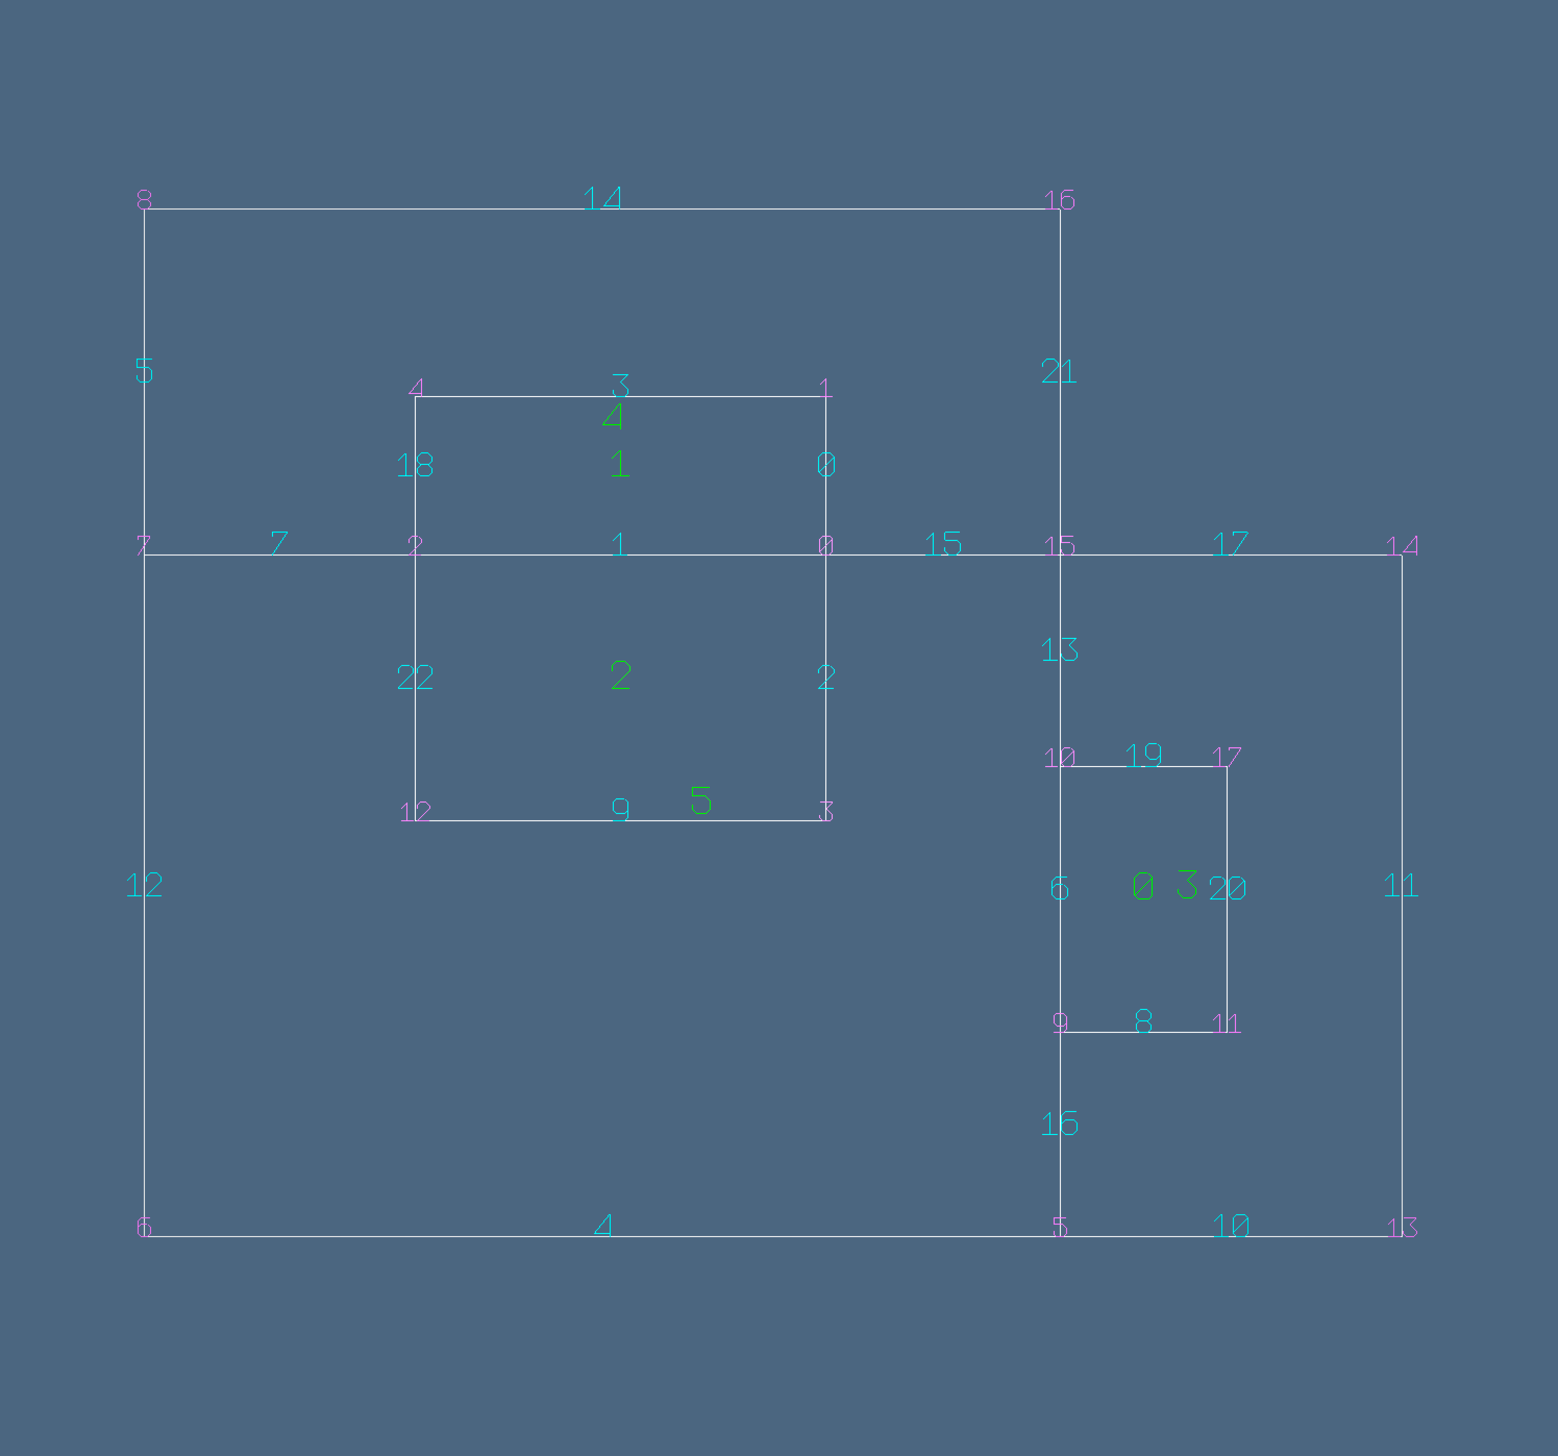
\includegraphics[height=0.245\linewidth,width=0.245\linewidth]{images/boundary-test02-02} 
   
\includegraphics[height=0.245\linewidth,width=0.245\linewidth]{images/boundary-test02-03} 
   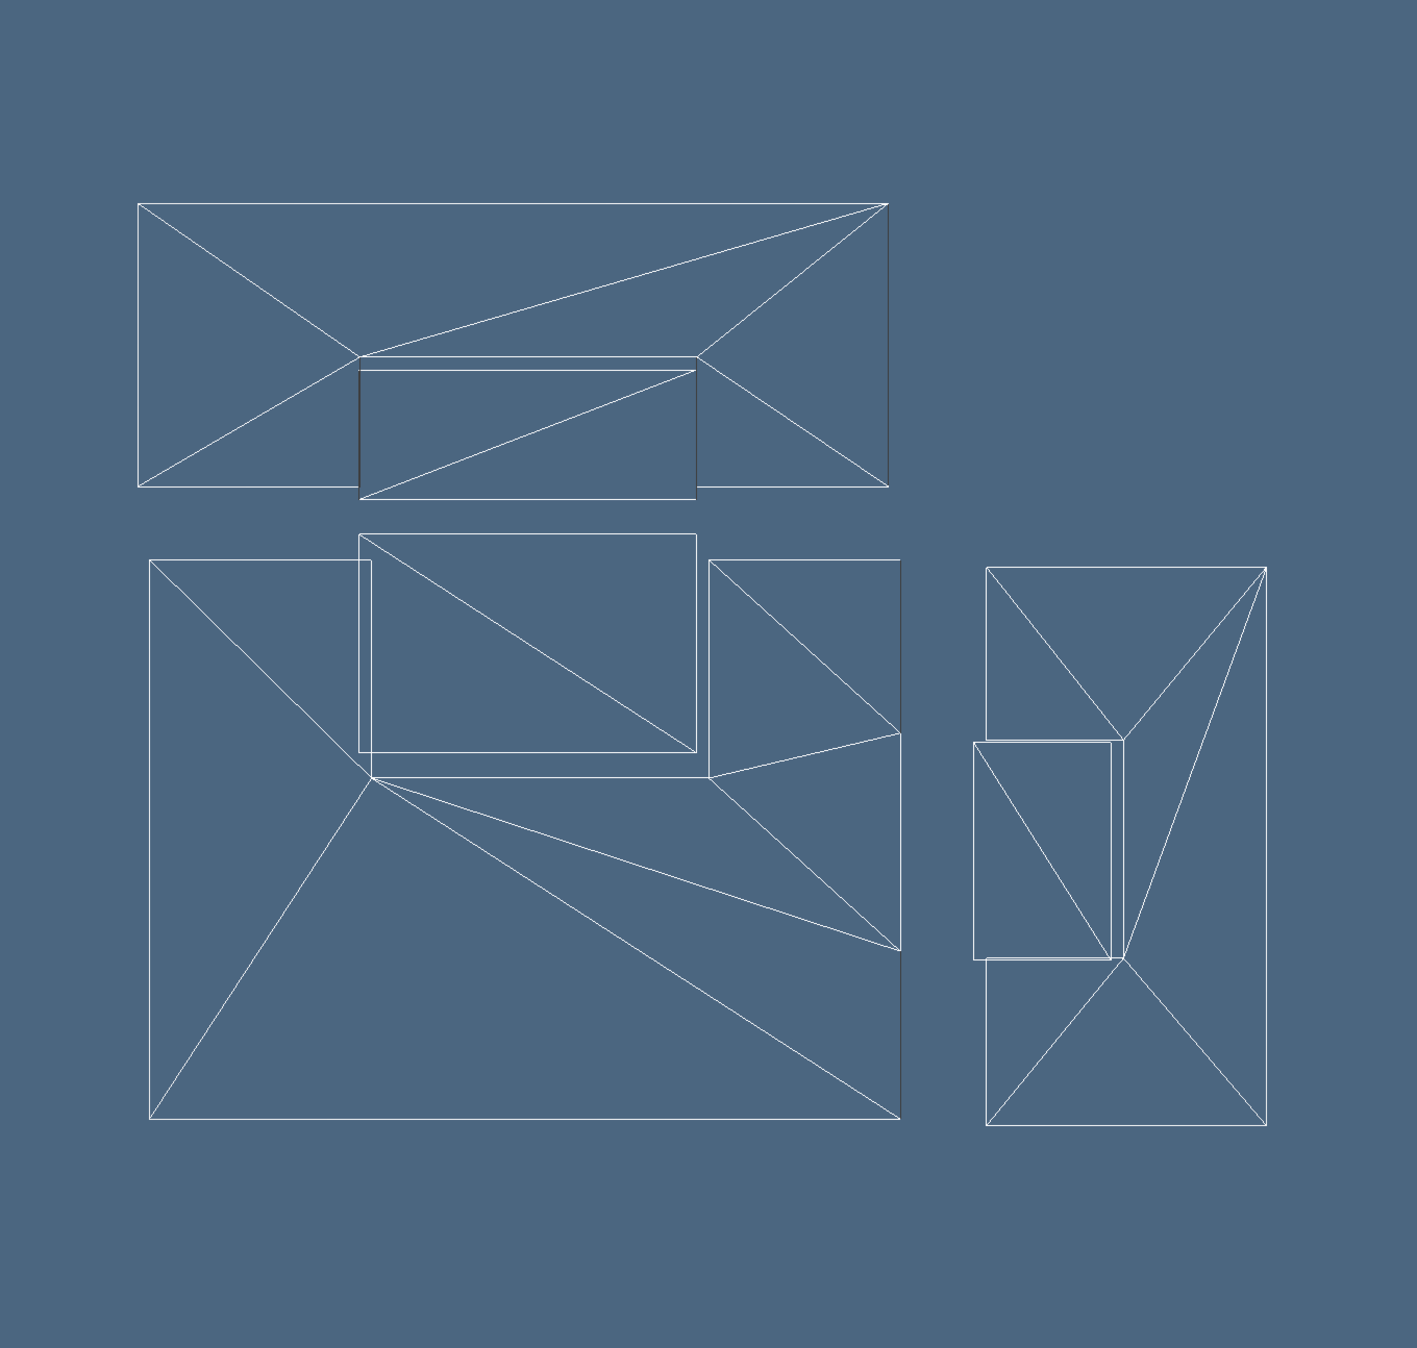
\includegraphics[height=0.245\linewidth,width=0.245\linewidth]{images/boundary-test02-04} 
   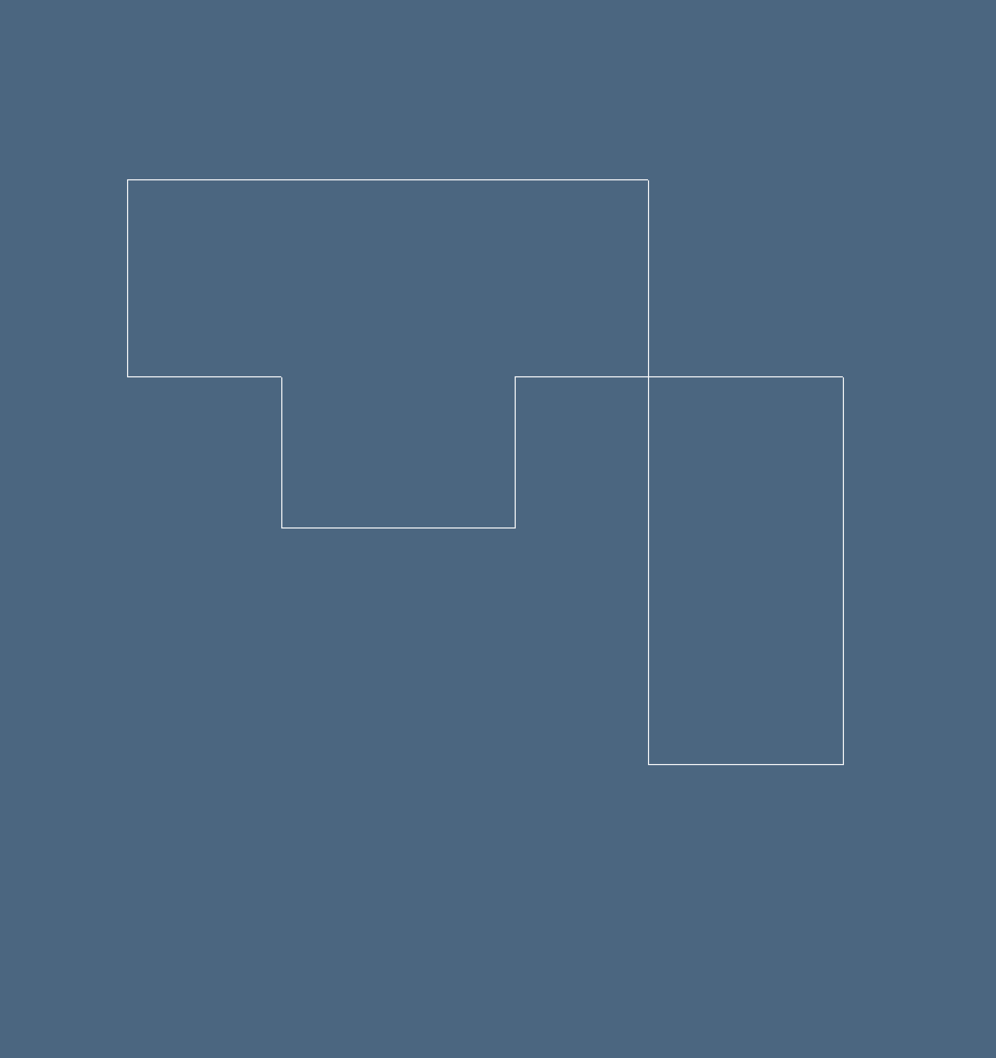
\includegraphics[height=0.245\linewidth,width=0.245\linewidth]{images/boundary-test02-05} 
   \caption{Non-convex LAR 2-complex with (two) 1-cells that are subsets of 2-cells without being their facets. Correctly disentangled by the \texttt{larUnsignedBoundary2()} function: (a) Indexing of 0-, 1-, and 2-cells; (b) exploded 2-cells; (c) triangulated and exploded 2-cells; (d) boundary of the 2-chain \texttt{[1,1,1,1,1,0]}.}
   \label{fig:example}
\end{figure}


%-------------------------------------------------------------------------------
@D From cells and facets to boundary cells
@{def totalChain(cells):
    return csr_matrix(len(cells)*[[1]])

def boundaryCells(cells,facets):
    csrBoundaryMat = larBoundary(cells,facets)
    csrChain = csr_matrix(totalChain(cells))
    csrBoundaryChain = csrBoundaryMat * csrChain
    out = [k for k,val in enumerate(csrBoundaryChain.data.tolist()) if val == 1]
    return out

def boundary2Cells(cells,facets,faces):
    csrBoundaryMat = larUnsignedBoundary2(cells,facets,faces)
    csrChain = csr_matrix(totalChain(cells))
    csrBoundaryChain = csrBoundaryMat * csrChain
    out = [k for k,val in enumerate(csrBoundaryChain.data.tolist()) if val == 1]
    return out

def boundary3Cells(cells,facets,faces):
    csrBoundaryMat = boundary3(cells,facets,faces)
    csrChain = csr_matrix(totalChain(cells))
    csrBoundaryChain = csrBoundaryMat * csrChain
    out = [k for k,val in enumerate(csrBoundaryChain.data.tolist()) if val == 1]
    return out
@}
%-------------------------------------------------------------------------------


\subsection{Correctness proof}

Our goal is to get a constructive and, of course, correct representation of the matrix $[\partial_3]$ starting only from $M_1$, $M_2$, and $M_3$.

We have sufficient evidence here to support the correctness of our identification of the matrices of boundary operators as discussed in the previous section. Remember that $M_1$, $M_2$, and $M_3$ are the characteristic matrices of 1-cells, 2-cells and 3-cells as subsets of vertices, and that $C_0, C_1, C_2, C_3$ are the linear spaces of 0-, 1-, 2-, and 3-chains, with coefficients in the field $\Z_2=\{0,1\}$.

In the following we give a dimension-independent proof, even our implementation is currently restricted to $d\in\{1,2,3\}$.

\paragraph{Preamble}
It is well known that a linear transformation $T: V\to W$ between two linear spaces, with fixed bases  of dimension $n$ and $m$ respectively, is represented uniquely by a matrix $A\in \R^{m\times n}$, that by columns contains the coordinate representations in $W$ of the basis vectors of $V$. 


\begin{theorem}
Consider the linear transformation $\partial_d: C_d \to C_{d-1}$. Having fixed the bases, made by singleton cells in $C_d$ and $C_{d-1}$, the transformation $\partial_d$ can be represented as a matrix product ${c} \mapsto [\partial_d]\, {c}$, where ${c}\in C_d$ is the coordinate representation of a d-chain, and $[\partial_d]$ is the $m\times n$ binary matrix having \emph{by columns} the coordinate representation in $C_{d-1}$ of the boundary $(d-1)$-chains of cells in $C_{d}$.
\end{theorem}

\begin{proof}
The computation of the boundary operator matrix $A_d = [\partial_d] \in\Z_2^{m\times n}$, where $m$ and $n$ are the dimensions of the linear spaces $C_d$ and $C_{d-1}$, respectively, is made in two steps, in the general case.

\paragraph{First step} 
Consider the characteristic matrices $M_d\in\Z_2^{m\times q}$ and $M_{d-1}\in\Z_2^{n\times q}$ having as rows the images of characteristic functions of bases elements as subsets of vertices, where $q$ is the number of vertices.

Then consider the product matrix $M=M_{d-1}M_{d}^t=(m_{ij})$, with values in the set $\N$ of non-negative integers. Clearly $m_{ij}$ will coincide with the number of vertices shared by cells $c_i\in C_{d-1}$ and $c_j\in C_d$, i.e. with the cardinality of their intersection as discrete sets of vertices. The predicate 
\begin{equation}
m_{ij} \equiv |c_i|
\label{eq:intersection}
\end{equation}
is a \emph{necessary} condition for $c_i$ to be a \emph{facet} of $c_j$. Using the Iverson bracket notation, where $[P]$ returns either 1 or 0 depending on the truth of predicate $P$, we can  assign (to) the $(i,j)$ element of our (tentative) boundary matrix the corresponding value:
\begin{equation}
A_d(i,j) := [m_{ij} \equiv |c_i|], \qquad 1\leq i\leq m,\, 1\leq j\leq n.
\label{eq:iverson}
\end{equation}
Unfortunately, condition~(\ref{eq:intersection}) is also \emph{sufficient} for $c_i$ being a facet of $c_j$ only when both are convex cells. In other words, Equation~(\ref{eq:iverson}) with $A_d=[\partial_d]$ holds in full generality if and only if the cellular complex under consideration is made only by convex cells. With more general cells, the column $j$ of the $\partial_d$ matrix contains the coordinate representation in $C_{d-1}$ of a possibly proper \emph{superset}  of $\partial_d(c_j)$.

\paragraph{Second step} 
In order to reduce the columns of the approximate boundary matrix $A_d$ to their exact value in $\Z_2^m$, with $m=\dim C_{d-1}$, we may compute an (approximate) matrix $B\in\N^{p\times n}$ of the operator $\partial_{d-1}\circ\partial_d: C_d \to C_{d-2}$, with $p=\dim C_{d-2}$, by using the approximate representation $A_d$ of the matrix $[\partial_d]$. Let us remark that the exact value of the latter is yet unknown at this point.

According to what asserted in the preamble, every column of this matrix should contain the coordinate representation (in $C_{d-2}$) of the boundary of the boundary of a basis element in $C_d$, i.e.~of a singleton $d$-chain.

Therefore, we will enforce the validity of the constraints $\partial\partial=0$, by checking
the values of columns in the product matrix $B_d = A_{d-1} A_d \in \N^{p\times n}$. In particular, ~every unit vector $e_j$, \emph{i.e.},~the coordinate representation of a singleton chain $c_j\in C_d$, should be mapped by $B_d$ to the zero vector in $\Z_2^p$:
\begin{equation}
e_j \mapsto B_d\, e_j = 0^{p} \in \Z_2^p, \qquad c_j\in C_d.
\label{eq:boundaryofboundary}
\end{equation}

Now, let consider the cells of LAR both as subsets of vertices and as cells of a cellular complex.
Actually, in the LAR general case, there may be some $(d-1)$-facets of some $d$-cell that are subsets of other $d$-cells of which they are not faces. It is not difficult to provide some examples of this fact (see Figure~\ref{fig:}).

When considering each column of $B$ as the coordinate representation of the boundary $(d-2)$-chain of a $d$-cell, and noting that every $d$-cell must be \emph{orientable}, and hence separating an interior space from an exterior space, we conclude that the number of occurrencies of each $(d-2)$-cell in a $B$ column must be necessarily even. In particular, it must be either equal to 2 if the column (the $d$-cell) is locally manifold, or equal to some even number $>2$ if the $d$-cell is locally non-manifold. But \emph{odd incidencies} of $(d-2)$-cells along the $d$-cell boundary \emph{are not allowed}. 

Therefore, for each column $B_j$ ($1\leq j\leq n$) we look for the subset of rows (i.e.~boundary $(d-2)$-faces of $c_j$) of odd value. If there are none, the column $A_j$, associated to $c_j$, is a correct representation of $[\partial_d]_j$. Otherways, we must look for the subsets of $(d-1)$-cells \emph{incorrectly} considered facets of $c_j$.

Let us call $R_j$ the subset of row indices corresponding to odd values in column $B_j$, and consider the subset of $A_j$ rows with value $a_{ij}=1$, i.e.~the superset $S_j$ of $(d-1)$-cells including the boundary $(d-1)$-chain of $c_j$. The redundant vertex subsets that are not boundary facets of $c_j$  are easily discovered by looking at the $(d-2)$-boundary of each $s\in S_j$.

In particular, the $(d-1)$-cell $s\in S_j$ is \emph{redundant} or \emph{extraneous} with respect to the $c_j$ boundary if and only if $\partial_{d-1}(s) \subseteq R_j$, because that property has certainly introduced a spurious increment for each $(d-2)$-facet in the count of incidences of boundary facets.

At this point, we can finally compute the actual boundary matrix $\partial_d$ for a \emph{general} LAR cellular complex, using again the Iverson brackets:
\begin{align*}
[\partial_d]_{ij} = [(a_{ij}=1) \wedge ((R_j=\emptyset) \vee (R_j \not\supseteq \partial_{d-1}(s_i)))]\qquad 1\leq i\leq m,\, 1\leq j\leq n
\end{align*}
In words it sounds that \emph{the element $(i,j)$ of the boundary matrix $[\partial]_d$ equals that of the ``approximate'' matrix $A_d$ if and only if either the redundant set $R_j$ is empty, or if it does not contain the $(d-1)$-boundary chain of the $i$-th $(d-1)$-cell.}

Just remember that the redundant set $R_j$ contains the $(d-2)$-faces with odd incidencies on $c_j\in C_d$, computed via the ``approximate'' matrix $B_d = A_{d-1}\circ A_d$.

\end{proof}  


\subsection{Oriented operators}

\subsubsection{Oriented simplicial complexes}

\subsubsection{Oriented LAR complexes}






\section{From relations to operators}
%===============================================================================

The LAR approach to topology, implemented in the \texttt{LarLib} modules, allows the user to consider the topological relations of incidence and adjacency between faces of a cellular complex as \emph{linear operators} between chains of cells of various dimensions. 

The previous approach was to consider the incidence and adjaceny as set-theoretical relations, to be solved by using typical database tools. Conversely, according to the novel IT evolution towards big data and cloud-based storage, even for geometrical data, \texttt{LarLib}  takes advantage of a conceptual framework based on linear-algebra and sparse matrices.

\subsection{Classification of operators} 

In the standard solid modeling approach, mainly based on boundary representations, the standard topological operations concern the answers to queries, by reporting the subsets of boundary elements which are incident (different dimension) or adjacent (equal dimension) to assigned boundary elements. Boundary elements stand there for three type of boundary cells: aka \emph{faces} $F$, \emph{edges} $E$, and \emph{vertices} $V$. Nine binary relations may be considered, that are summarized in Table~\ref{tab:one}.
\begin{table}[htbp]
\caption{Binary topological relations between boundary elements in boundary representations of solid models}
\begin{center}
\begin{tabular}{|c|ccc|}
\hline 
  & F & E & V \\
\hline 
F & FF & FE & FV \\
E & EF & EE & EV \\
V & VF & VE & VV \\
\hline 
\end{tabular}
\end{center}
\label{tab:one}
\end{table}%

Conversely, LAR  models are normally based on cellular 3-complexes, so using four sets of cells, namely \emph{3-cells} $C$, \emph{2-cells} $F$, \emph{1-cells} $E$, and \emph{0-cells} $V$. The resulting tables of topological relations, and the associated linear operators, are shown in Tables~\ref{tab:two}a and \ref{tab:two}b, respectively.
\begin{table}[htbp]
\caption{Binary topological relations between cells of LAR decompositions of  solid models and corresponding topological operators on $\partial_\circ$ chains.}
\vspace{3mm}
\begin{minipage}[c]{0.5\linewidth}\centering
\begin{tabular}{|c|cccc|}
\hline 
  & C & F & E & V \\
\hline 
C & CC & \fbox{CF} & \fbox{CE} & CV \\
F & \fbox{FC} & FF & \fbox{FE} & FV \\
E & \fbox{EC} & \fbox{EF} & EE & EV \\
V & VC & VF & VE & VV \\
\hline 
\end{tabular}
\end{minipage}
\begin{minipage}[c]{0.5\linewidth}\centering
\begin{tabular}{|c|cccc|}
\hline 
  & C & F & E & V \\
\hline 
C & $\v{1}_C^\top\circ\v{1}_C$ & {$\partial_3$} & {$\partial_2\circ\partial_3$} & $\v{1}_C$ \\
F & {$\delta_2$} & $\v{1}_F^\top\circ\v{1}_F$ & {$\partial_2$} & $\v{1}_F$ \\
E & {$\delta_2\circ\delta_1$} & {$\delta_1$} & $\v{1}_E^\top\circ\v{1}_E$ & $\v{1}_E$ \\
V & $\v{1}_C^\top$ & $\v{1}_F^\top$ & $\v{1}_E^\top$ & $\v{1}_V$ \\
\hline 
\end{tabular}
\end{minipage}
\label{tab:two}
\end{table}%

\subsection{Topological relations}
%~~~~~~~~~~~~~~~~~~~~~~~~~~~~~~~~~~~~~~~~~~~~~~~~~~~~~~~~~~~~~~~~~~~~~~~~~~~~~~~~



\subsubsection{Adjacency relations}

%-------------------------------------------------------------------------------
@D kfaces-to-kfaces relation
@{""" kfaces-to-kfaces relation """
eeOp = larEdges2Edges(EV,VV)
EE = [eeOp([k]) for k in range(len(EV))]

ffOp = larFaces2Faces(FV,EV)
FF = [ffOp([k]) for k in range(len(FV))]

ccOp = larCells2Cells(CV,FV,EV)
CC = [ccOp([k]) for k in range(len(CV))]

@}
%-------------------------------------------------------------------------------

\paragraph{Adjacency relations examples}
%-------------------------------------------------------------------------------
@O test/py/boundary/test09.py
@{""" Adjacency relations examples """
from larlib import *

sys.path.insert(0, 'test/py/boundary/')
from test07 import *

@< kfaces-to-kfaces relation @>
print "\nCC =",CC
print "\nFF =",FF
print "\nEE =",EE,"\n"

V,BF,BE = larUnsignedBoundary3(V,CV,FV,EV)([1,0])
VIEW(STRUCT(MKTRIANGLES((V,[FV[h] for h in FF[-1]],EV),color=True)))
VIEW(STRUCT(MKPOLS((V,[EV[h] for h in EE[-1]]))+[COLOR(RED)(MKPOLS((V,[EV[-1]]))[0])]))
@}
%-------------------------------------------------------------------------------


\subsubsection{Incidence relations}

%-------------------------------------------------------------------------------
@D mfaces-to-nfaces relations
@{""" mfaces-to-nfaces relations """
fcOp = larCells2Faces(CV,FV,EV)
CF = [fcOp([k]) for k in range(len(CV))]
FC = invertRelation(CF)

ecOp = larCells2Edges(CV,FV,EV)
CE = [ecOp([k]) for k in range(len(CV))]
EC = invertRelation(CE)
    
efOp = larFaces2Edges(FV,EV)
FE = [efOp([k]) for k in range(len(FV))]
EF = invertRelation(FE)
@}
%-------------------------------------------------------------------------------

\paragraph{Incidence relations examples}
%-------------------------------------------------------------------------------
@O test/py/boundary/test10.py
@{""" Incidence relations examples """
from larlib import *

sys.path.insert(0, 'test/py/boundary/')
from test08 import *

@< mfaces-to-nfaces relations @>
print "\nFC =",FC
print "\nEC =",EC
print "\nEF =",EF,"\n"
@}
%-------------------------------------------------------------------------------





\subsection{Querying}
%~~~~~~~~~~~~~~~~~~~~~~~~~~~~~~~~~~~~~~~~~~~~~~~~~~~~~~~~~~~~~~~~~~~~~~~~~~~~~~~~

The more important topological operations in a geometric system concern the answer to queries of the type: ``what is the $h$-chain whose cells are $(k-h)$-incident to a given $h$-chain''?

An efficient answer is given by the three higher-level functions in this section, respectively denoted as \texttt{larCells2Faces}, \texttt{larCells2Edges}, and \texttt{larFaces2Edges}.
Their first application, over the two or three necessary (compressed) characteristic matrices, returns the \texttt{csr\_matrix} of the topological operator, that can be so cached by the calling code.
The second application, over the list of $h$-chain indices, returns the list of $k$-chain indices of the cells that share with them a $(k-h)$-face.


\subsubsection{Topological incidences}


\paragraph{Query from 3-chain to incident 2-chain}
%-------------------------------------------------------------------------------
@D Query from 3-chain to incident 2-chain
@{""" Query from 3-chain to incident 2-chain """
def larCells2Faces(CV,FV,EV):
    csrFC = boundary3(CV,FV,EV)
    def larCells2Faces0(chain):
        chainCoords = csc_matrix((csrFC.shape[1],1),dtype='b')
        for k in chain: chainCoords[k,0] = 1
        out = csrFC * chainCoords
        return out.tocoo().row.tolist()
    return larCells2Faces0
@}
%-------------------------------------------------------------------------------

\paragraph{Query from 3-chain to incident 1-chain}
%-------------------------------------------------------------------------------
@D Query from 3-chain to incident 1-chain
@{""" Query from 3-chain to incident 1-chain """
def larCells2Edges(CV,FV,EV):
    lenV = max(CAT(CV))+1
    VV = AA(LIST)(range(lenV))
    csrEC = larUnsignedBoundary2(FV,EV,VV) * boundary3(CV,FV,EV)
    def larCells2Faces0(chain):
        chainCoords = csc_matrix((csrEC.shape[1],1),dtype='b')
        for k in chain: chainCoords[k,0] = 1
        out = csrEC * chainCoords
        return out.tocoo().row.tolist()
    return larCells2Faces0
@}
%-------------------------------------------------------------------------------


\paragraph{Compute the signed 2-boundary matrix}
Compute the signed 2-boundary matrix. The second definition extends the first one by considering LAR faces including holes. For this purpose the signed areas of all loops inside each lar face in FV are taken into account, and only the greates positive area and all the negative areas (exept the most negative one) are considered. 
%-------------------------------------------------------------------------------
@D Compute the signed 2-boundary matrix
@{""" Compute the signed 2-boundary matrix """
import triangulation,integr
    
def larSignedBoundary2(V,FV,EV):
    efOp = larFaces2Edges(V,FV,EV)
    FE = [efOp([k]) for k in range(len(FV))]
    data,row,col = [],[],[]
    for f in range(len(FE)):
            
        Vcycles,Ecycles = triangulation.makeCycles((V,[EV[e] for e in FE[f]]))
        Ecycles = [[FE[f][e] for e in cycle] for cycle in Ecycles]
        areas = integr.signedSurfIntegration((V,Vcycles,EV),signed=True)
        sortedAreas = sorted((area,k) for k,area in enumerate(areas))
        innerLoops = [zip(Vcycles[k],Ecycles[k]) for area,k in sortedAreas[1:] if area<0]
        outerLoop = [zip(Vcycles[sortedAreas[-1][1]],Ecycles[sortedAreas[-1][1]])]
        orientedFaceLoops = CAT(outerLoop+innerLoops)
        coefficients = [1 if v==EV[e][0] else -1 for v,e in orientedFaceLoops]
		
        ecycle = [e for v,e in orientedFaceLoops]
        data += coefficients
        row += ecycle
        col += [f]*len(ecycle)
        #print f,len(data),len(row),len(col)
    signedBoundary2 = coo_matrix((data,(row,col)), shape=(len(EV),len(FV)),dtype='b')
    return csr_matrix(signedBoundary2)
@}
%-------------------------------------------------------------------------------


\paragraph{Compute any signed 1-boundary chain}
The script below computes the signed boundary 1-cycle of any 2-chain in a 2-complex. 
The script returns the pair of arrays \texttt{orientations,boundaryCells}, providing the signs of 1-cells in the extracted 1-cycle and their edge indices, respectively.
%-------------------------------------------------------------------------------
@D Compute any signed 1-boundary chain
@{""" Compute any signed 1-boundary chain """
def larSignedBoundary2Cells(V,FV,EV):
	def larSignedBoundary2Cells0(chain):
		boundaryMat = larSignedBoundary2(V,FV,EV)
		chainCoords = csc_matrix((len(FV), 1))
		for cell in chain: chainCoords[cell,0] = 1
		boundaryCells = list((boundaryMat * chainCoords).tocoo().row)
		orientations = list((boundaryMat * chainCoords).tocoo().data)
		return orientations,boundaryCells
	return larSignedBoundary2Cells0
@}
%-------------------------------------------------------------------------------


\paragraph{Testing the extraction of a boundary chain}
An example for testing the extraction of the boundary 1-cycle of a 2-chain $[f_1,f_2]$ is given below.
The images generated by the script are displayed in Figure~\ref{fig:signedBoundary2}.
%-------------------------------------------------------------------------------
@O test/py/boundary/test14.py
@{""" Testing the extraction of a boundary chain """
from larlib import *

lines = svg2lines("test/svg2lines/test.svg")
V,FV,EV,polygons = larFromLines(lines,True)
VIEW(STRUCT(MKTRIANGLES((V,FV,EV),color=True)))
submodel = mkSignedEdges((V,EV))
VV = AA(LIST)(range(len(V)))
VIEW(larModelNumbering(1,1,1)(V,[VV,EV,FV],submodel,0.25))

orientations,boundaryCells = larSignedBoundary2Cells(V,FV,EV)([1,2])
orientedBoundaryCells = [EV[e] if sign==1 else REVERSE(EV[e]) 
						for sign,e in zip(orientations,boundaryCells)]

VIEW(STRUCT(MKTRIANGLES((V,FV[1:3],EV),color=True)))
VIEW(mkSignedEdges((V,orientedBoundaryCells)))
@}
%-------------------------------------------------------------------------------



\begin{figure}[htbp] %  figure placement: here, top, bottom, or page
   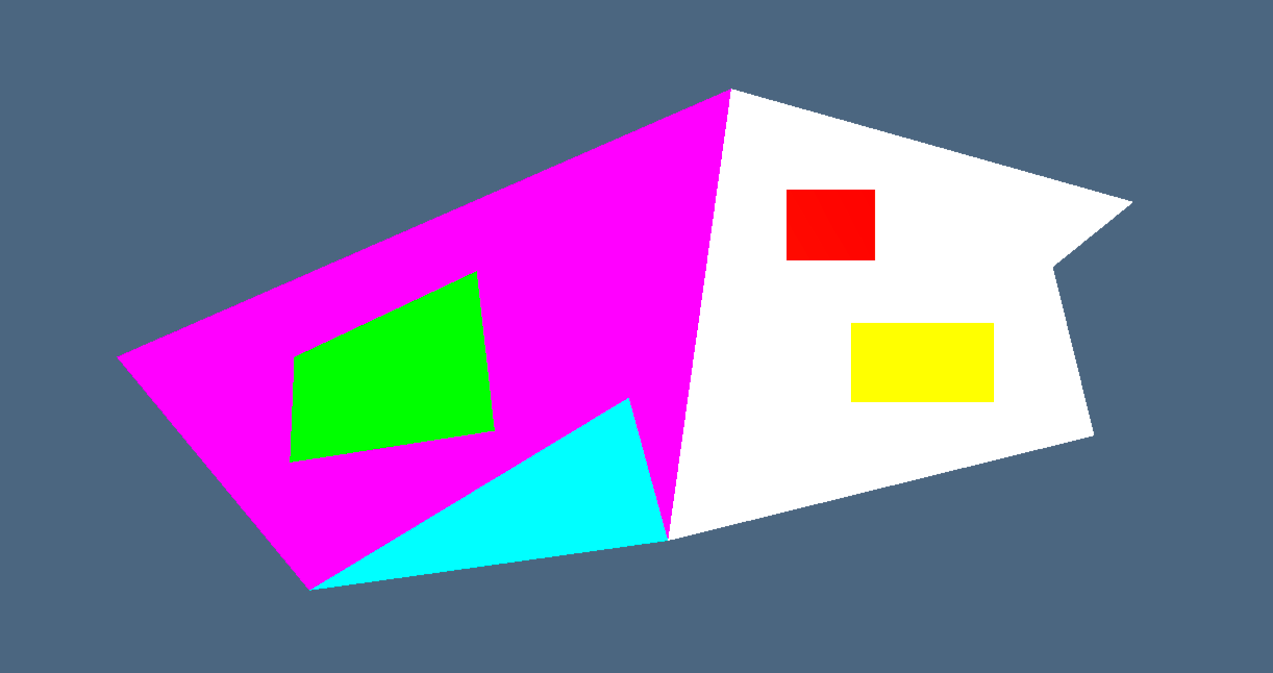
\includegraphics[height=0.27\linewidth,width=0.495\linewidth]{images/larSignedBoundary2a} 
   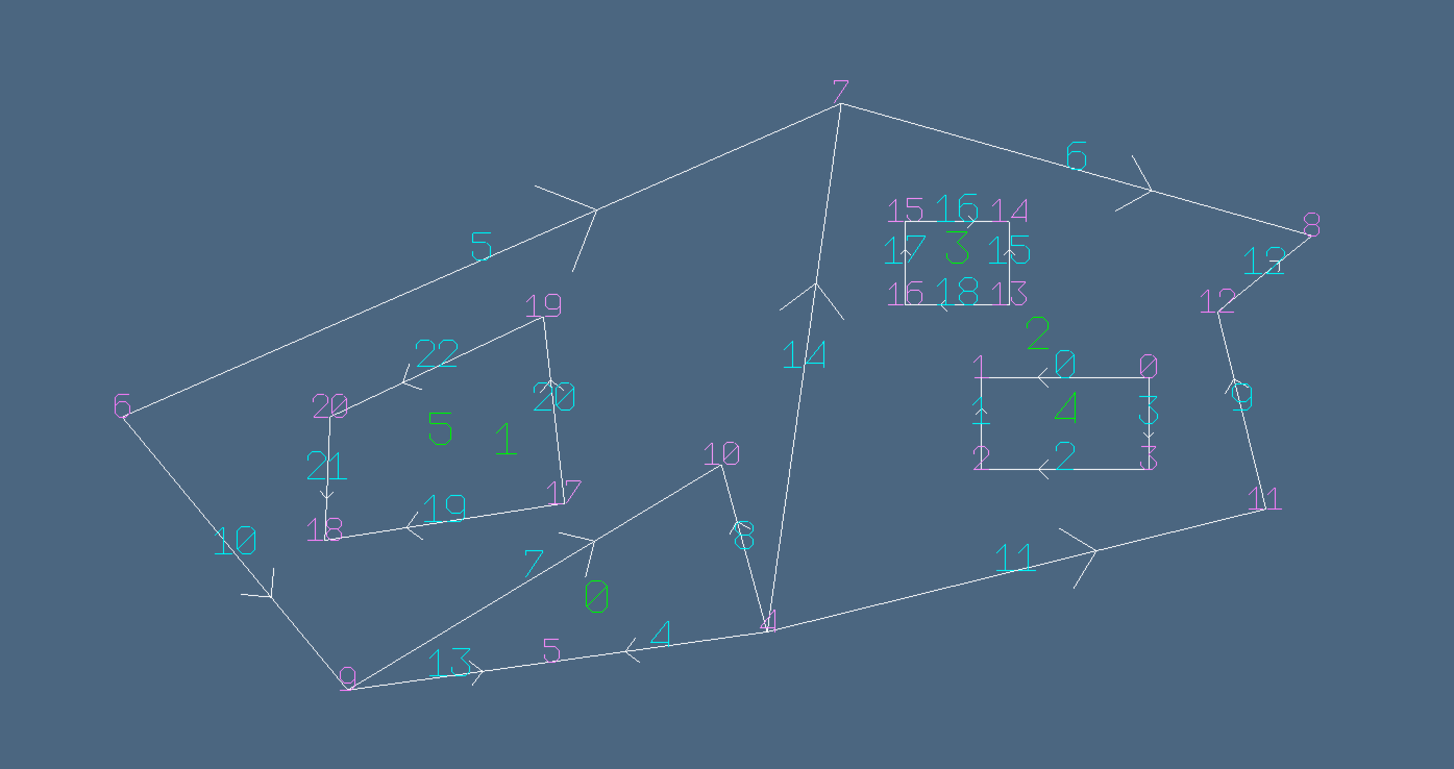
\includegraphics[height=0.27\linewidth,width=0.495\linewidth]{images/larSignedBoundary2b} 
   
   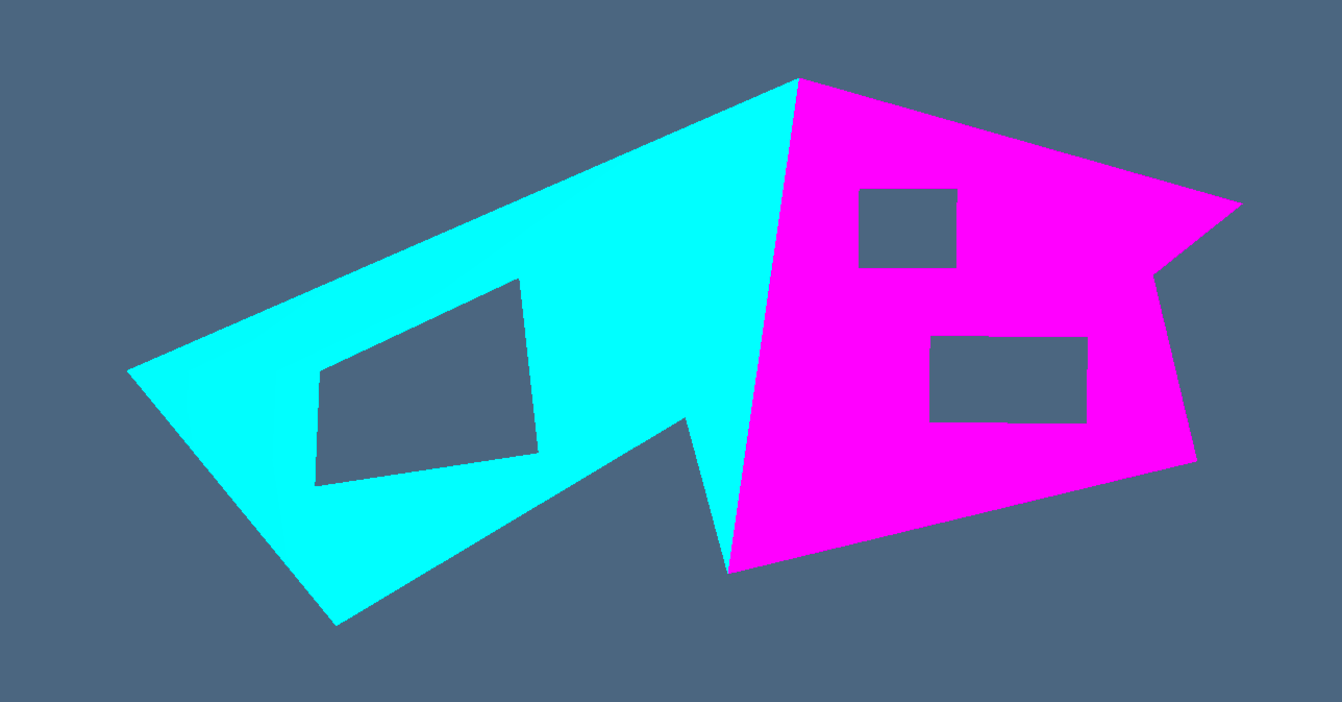
\includegraphics[height=0.27\linewidth,width=0.495\linewidth]{images/larSignedBoundary2c} 
   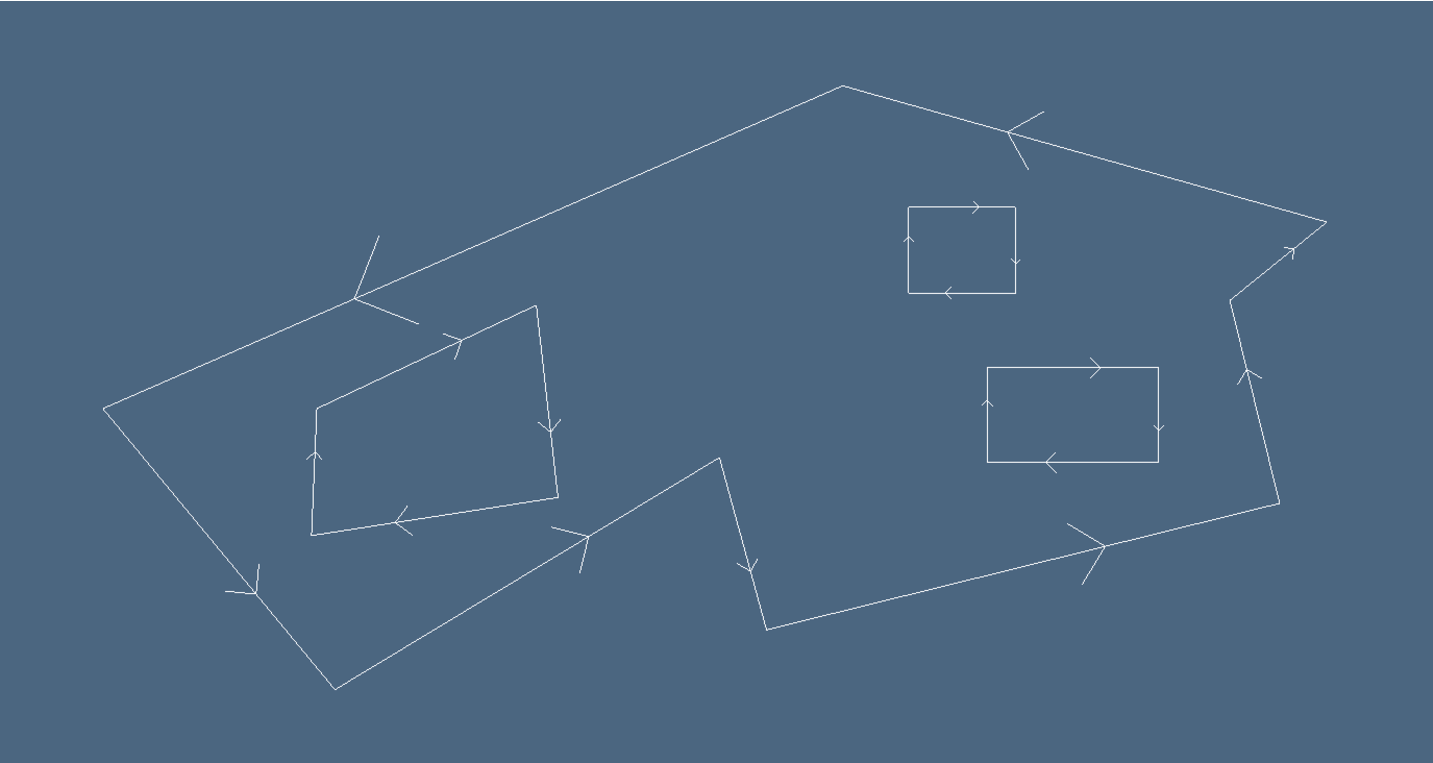
\includegraphics[height=0.27\linewidth,width=0.495\linewidth]{images/larSignedBoundary2d} 
   \caption{Example  of \emph{signed} boundary operator: (a) 2-complex with non-compressible cells; (b) oriented 1-cells; (c) drawing of the 2-chain $[f_1,f_2]$; (d) oriented boundary 1-chain of 2-chain $[f_1,f_2]$.}
   \label{fig:signedBoundary2}
\end{figure}


\paragraph{Query from 2-chain to incident 1-chain}
%-------------------------------------------------------------------------------
@D Query from 2-chain to incident 1-chain
@{""" Query from 2-chain to incident 1-chain """
def larFaces2Edges(V,FV,EV):
    VV = AA(LIST)(range(len(V)))
    csrEF = larUnsignedBoundary2(FV,EV,VV)
    def larCells2Faces0(chain):
        chainCoords = csc_matrix((csrEF.shape[1],1),dtype='b')
        for k in chain: chainCoords[k,0] = 1
        out = csrEF * chainCoords
        return out.tocoo().row.tolist()
    return larCells2Faces0
@}
%-------------------------------------------------------------------------------



\subsubsection{Topological adjacencies}

\paragraph{kfaces-to-kfaces relations}
%-------------------------------------------------------------------------------
@D kfaces-to-kfaces relations
@{""" kfaces-to-kfaces relations """

def larCells2Cells(CV,FV,EV):
    csrMat = boundary3(CV,FV,EV)
    csrCC = csrMat.T * csrMat
    def larCells2Cells0(chain):
        chainCoords = csc_matrix((csrCC.shape[1],1),dtype='b')
        for k in chain: chainCoords[k,0] = 1
        out = csrCC * chainCoords
        return out.tocoo().row.tolist()
    return larCells2Cells0

def larFaces2Faces(FV,EV):
    lenV = max(CAT(FV)) + 1
    VV = AA(LIST)(range(lenV))
    csrMat = larUnsignedBoundary2(FV,EV,VV)
    csrFF = csrMat.T * csrMat
    def larFaces2Faces0(chain):
        chainCoords = csc_matrix((csrFF.shape[1],1),dtype='b')
        for k in chain: chainCoords[k,0] = 1
        out = csrFF * chainCoords
        return out.tocoo().row.tolist()
    return larFaces2Faces0

def larEdges2Edges(EV,VV):
    lenV = len(VV)
    csrMat = larBoundary(EV,VV)
    csrEE = csrMat.T * csrMat
    def larFaces2Faces0(chain):
        chainCoords = csc_matrix((csrEE.shape[1],1),dtype='b')
        for k in chain: chainCoords[k,0] = 1
        out = csrEE * chainCoords
        return out.tocoo().row.tolist()
    return larFaces2Faces0
@}
%-------------------------------------------------------------------------------



\subsection{Oriented operators}

\subsubsection{Signed 2-boundary}



\paragraph{Testing signed 2-boundary}
%-------------------------------------------------------------------------------
@O test/py/boundary/test11.py
@{""" Testing signed 2-boundary """
from larlib import *

sys.path.insert(0, 'test/py/boundary/')
from test10 import *

@< mfaces-to-nfaces relations @>

signedBoundary2 = larSignedBoundary2(FV,EV)
@}
%-------------------------------------------------------------------------------


\paragraph{Testing signed 2-boundary}
%-------------------------------------------------------------------------------
@O test/py/boundary/test13.py
@{""" Testing signed 2-boundary """
from larlib import *

lines = svg2lines("test/svg2lines/test.svg")
V,FV,EV,polygons = larFromLines(lines,True)
VIEW(STRUCT(MKTRIANGLES((V,FV,EV),color=True)))
submodel = mkSignedEdges((V,EV))
VV = AA(LIST)(range(len(V)))
VIEW(larModelNumbering(1,1,1)(V,[VV,EV,FV],submodel,0.25))

B = larSignedBoundary2(V,FV,EV)
for k in range(B.shape[0]):
    print k,B.todense()[k]

VIEW(STRUCT(MKTRIANGLES((V,FV[1:3],EV),color=True)))
@}
%-------------------------------------------------------------------------------

\paragraph{Example 2-bondary matrix}
The example in file \texttt{test13.py}, corresponding to Figure~\ref{fig:signedBoundary2} produces the following two-dimensional LAR model:
{\scriptsize
\begin{verbatim}
V = [[0.8627, 0.263], [0.7223, 0.263], [0.7223, 0.1857], [0.8627, 0.1857], [0.5422, 0.0489], [0.3613, 
0.0238], [0.0, 0.2296], [0.6044, 0.4933], [1.0, 0.382], [0.1896, 0.0], [0.5037, 0.1896], [0.9614, 
0.1522], [0.9207, 0.318], [0.7457, 0.3241], [0.7457, 0.3942], [0.6583, 0.3942], [0.6583, 0.3241], 
[0.3718, 0.157], [0.1704, 0.1259], [0.3541, 0.3141], [0.1748, 0.2296]] 
EV = [[0, 1], [2, 1], [3, 2], [0, 3], [4, 5], [6, 7], [7, 8], [9, 10], [4, 10], [11, 12], [6, 9], 
[4, 11], [12, 8], [9, 5], [4, 7], [13, 14], [15, 14], [16, 15], [13, 16], [17, 18], [17, 19], 
[20, 18], [19, 20]]
\end{verbatim}}
and the following boundary operator matrix:
\[
\partial_2 =
\mat{ 
 0 & 0 &-1 & 0 & 1 & 0 \\
 0 & 0 & 1 & 0 &-1 & 0 \\
 0 & 0 & 1 & 0 &-1 & 0 \\
 0 & 0 & 1 & 0 &-1 & 0 \\
-1 & 0 & 0 & 0 & 0 & 0 \\
 0 &-1 & 0 & 0 & 0 & 0 \\
 0 & 0 &-1 & 0 & 0 & 0 \\
-1 & 1 & 0 & 0 & 0 & 0 \\
 1 &-1 & 0 & 0 & 0 & 0 \\
 0 & 0 & 1 & 0 & 0 & 0 \\
 0 & 1 & 0 & 0 & 0 & 0 \\
 0 & 0 & 1 & 0 & 0 & 0 \\
 0 & 0 & 1 & 0 & 0 & 0 \\
 1 & 0 & 0 & 0 & 0 & 0 \\
 0 & 1 &-1 & 0 & 0 & 0 \\
 0 & 0 &-1 & 1 & 0 & 0 \\
 0 & 0 & 1 &-1 & 0 & 0 \\
 0 & 0 & 1 &-1 & 0 & 0 \\
 0 & 0 & 1 &-1 & 0 & 0 \\
 0 & 1 & 0 & 0 & 0 &-1 \\
 0 &-1 & 0 & 0 & 0 & 1 \\
 0 &-1 & 0 & 0 & 0 & 1 \\
 0 &-1 & 0 & 0 & 0 & 1 \\
 }
\]


\paragraph{Transformation from chain coordinates to explicit chain data}
%-------------------------------------------------------------------------------
@D Transformation from chain coordinates to explicit chain data
@{""" Transformation from chain coordinates to explicit chain data """
def coords2chain(chainCoords):
    coo = coo_matrix(chainCoords)
    return [(e,val) for e,val in zip(coo.row,coo.data)]
@}
%-------------------------------------------------------------------------------


\subsection{Offset of 2-faces of a 2D complex}
In some applications it is necessary to compute the offset of faces of a 2D complex. This may happen for example in architectural applications, where the walls of building layout must be computed from its wire-frame design. Another important application aims to make more numerically robust the point-in-polygon containment test. In this case the test is driven against a slightly ``grown'' version of the polygon.
The problem solved by the \texttt{larOffset2D (model)} function given below is to "enlarge" each 2-face of a 2-complex in 2D of a (generally small) constant offset.  
For this purpose, the \texttt{larOffset2D} function operates as follows:

\begin{enumerate}
\item translate every 1-face towards its cobounday exterior (see Figure 1);
\item compute the parametric line equation for the translated pairs of edge vertices;
\item compute the intersection points between of adjacent pairs of such lines:
    \begin{enumerate}
    \item solving for both parameters;
    \item using the computed parameter value to get the intersection point.
    \end{enumerate}
\end{enumerate}
	
\paragraph{Offset of 2-faces of a 2D complex}
The coding below is using the Cramer's formula for the the solution of the intersection of two 2D lines via their parametric equation, according to page 50-51 of the formulation given in \href{http://www.ti.inf.ethz.ch/ew/lehre/CG09/materials/v9.pdf}{http://www.ti.inf.ethz.ch/ew/lehre/CG09/materials/v9.pdf}.
The implementation is  simple and very general---e.g.˜it does not require conditional constructs---so that it may be useful to avoid, for future GPGPU implementations.
%-------------------------------------------------------------------------------
@D Offset of 2-faces of a 2D complex
@{""" Offset of 2-faces of a 2D complex """
from scipy.linalg.basic import det

def larOffset2D (model,offset=0.001):
    V,FV,EV = model
    newVertices,lines = [],[]

    for f in range(len(FV)):
        # pair of arrays (signs, edges) of f face
        orientations,boundaryCells = larSignedBoundary2Cells(V,FV,EV)([f])
        # array of pairs (sign, edge) of f face
        edges = zip(orientations,boundaryCells)
        
        # array of pairs (begin_vertex, end_vertex) of oriented edges of f face
        orientedEdges = [tuple(EV[e]) if sign==1 else tuple(REVERSE(EV[e])) 
            for sign,e in edges]
        # array of unit tangentVectors of  f face
        tangentVectors = [UNITVECT(VECTDIFF([ V[edge[1]],V[edge[0]] ])) 
            for edge in orientedEdges]
        # array of unit normalVectors of   f face
        normalVectors = [ SCALARVECTPROD([ offset,[vect[1],-vect[0]] ]) 
            for vect in tangentVectors]
        # array of pairs of moved vertices  of oriented edges of f face
        movedEdgesOffLine = [[VECTSUM([V[v],n]) for v in orientedEdges[k]] 
            for k,n in enumerate(normalVectors)]
        # successor map ( succ[first] := second ) for verts of oriented edges of $f$ 
        succ = dict(orientedEdges)
        # dictionary of numerals of oriented edges of $f$ (key = pair of vertices)
        edgeDict = dict([(edge,k) for k,edge in enumerate(orientedEdges)])
        # array of pairs of numerals of intersecting edges
        intersections = [[ edgeDict[(u,v)], edgeDict[(v,succ[v])] ] 
            for k,(u,v) in enumerate(orientedEdges)]
        # coupling of data points of intersecting pairs
        linepairs = [[movedEdgesOffLine[l1],movedEdgesOffLine[l2]] 
            for l1,l2 in intersections]
        # prepare data for line pairs
        linedata = [[ax,ay,bx,by,cx,cy,dx,dy] 
            for [[(ax,ay),(bx,by)],[(cx,cy),(dx,dy)]] in linepairs]
        # assemble intersection determinants
        determinants = [ det(mat([[ax-bx,dx-cx], [ay-by,dy-cy]])) 
            for [ax,ay,bx,by,cx,cy,dx,dy] in linedata]
        # parameter pairs by Cramer's rule (for oriented edges of f face)
        alpha = [det(mat([[dx-bx,dx-cx],[dy-by,dy-cy]]))/D  if abs(D)>.00001 else 0 
            for D,(ax,ay,bx,by,cx,cy,dx,dy) in zip(determinants,linedata)]
        # intersection points
        newvert = [ (a*mat(p1)+(1-a)*mat(p2)).tolist()[0] 
            for a,[[p1,p2],[q1,q2]] in zip(alpha,linepairs)]
        newedges = [[newvert[u],newvert[v]] for u,v in intersections]

        newVertices += [newvert]
        lines += newedges  
    return lines

@}
%-------------------------------------------------------------------------------


\paragraph{Example of Offset generation for the 2-faces of a 2D complex}
The result of execution of the test program below is given in Figure˜\ref{fig:offset}
%-------------------------------------------------------------------------------
@O test/py/boundary/test15.py
@{""" Example of Offset generation for the 2-faces of a 2D complex """
from larlib import *
lines = svg2lines("test/svg2lines/test.svg")
V,FV,EV,polygons = larFromLines(lines,True)
VIEW(STRUCT(MKTRIANGLES((V,FV,EV),color=True)))

submodel = mkSignedEdges((V,EV))
VV = AA(LIST)(range(len(V)))
VIEW(larModelNumbering(1,1,1)(V,[VV,EV,FV],submodel,0.25))

newEdges = larOffset2D((V,FV,EV),offset=0.01)
VIEW(STRUCT(MKPOLS((V,EV)) + AA(COLOR(YELLOW))(AA(POLYLINE)(newEdges))))
@}
%-------------------------------------------------------------------------------

\begin{figure}[htbp] %  figure placement: here, top, bottom, or page
   \centering
   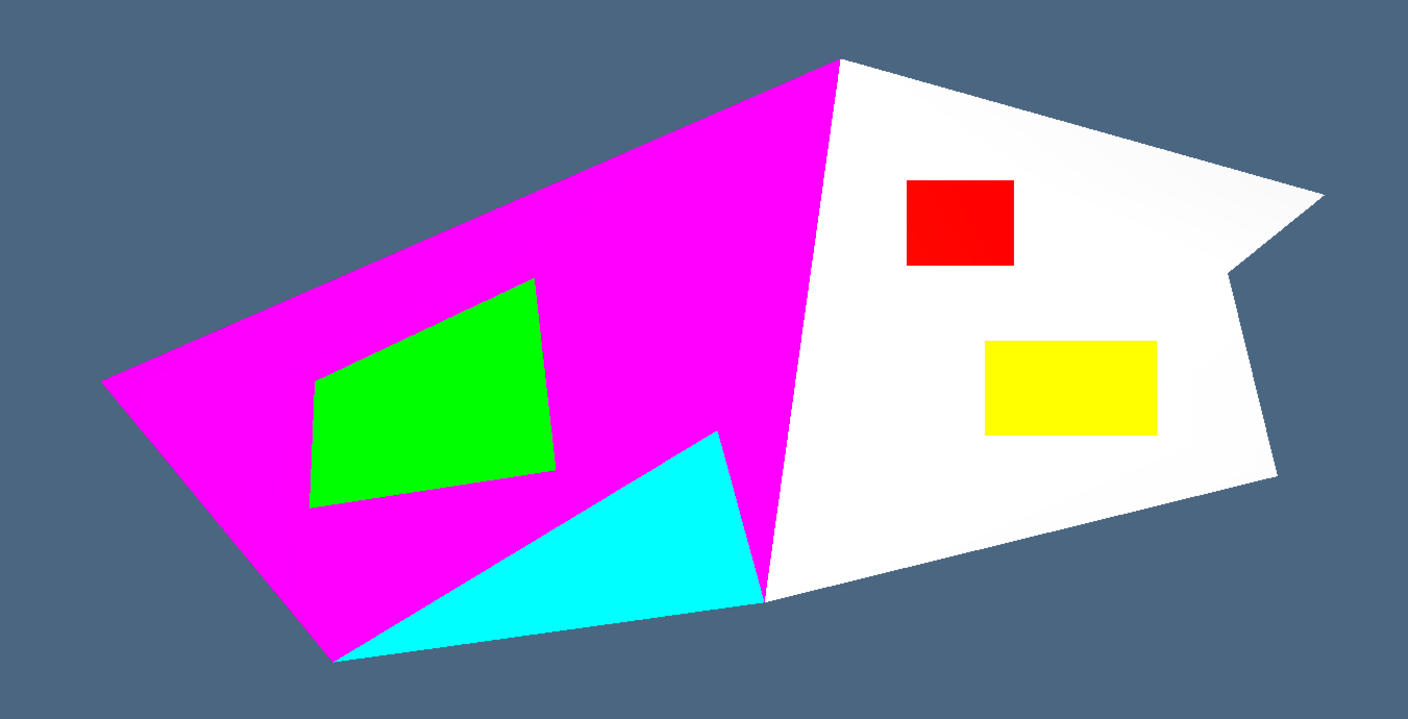
\includegraphics[width=0.49\linewidth]{images/offset1} 
   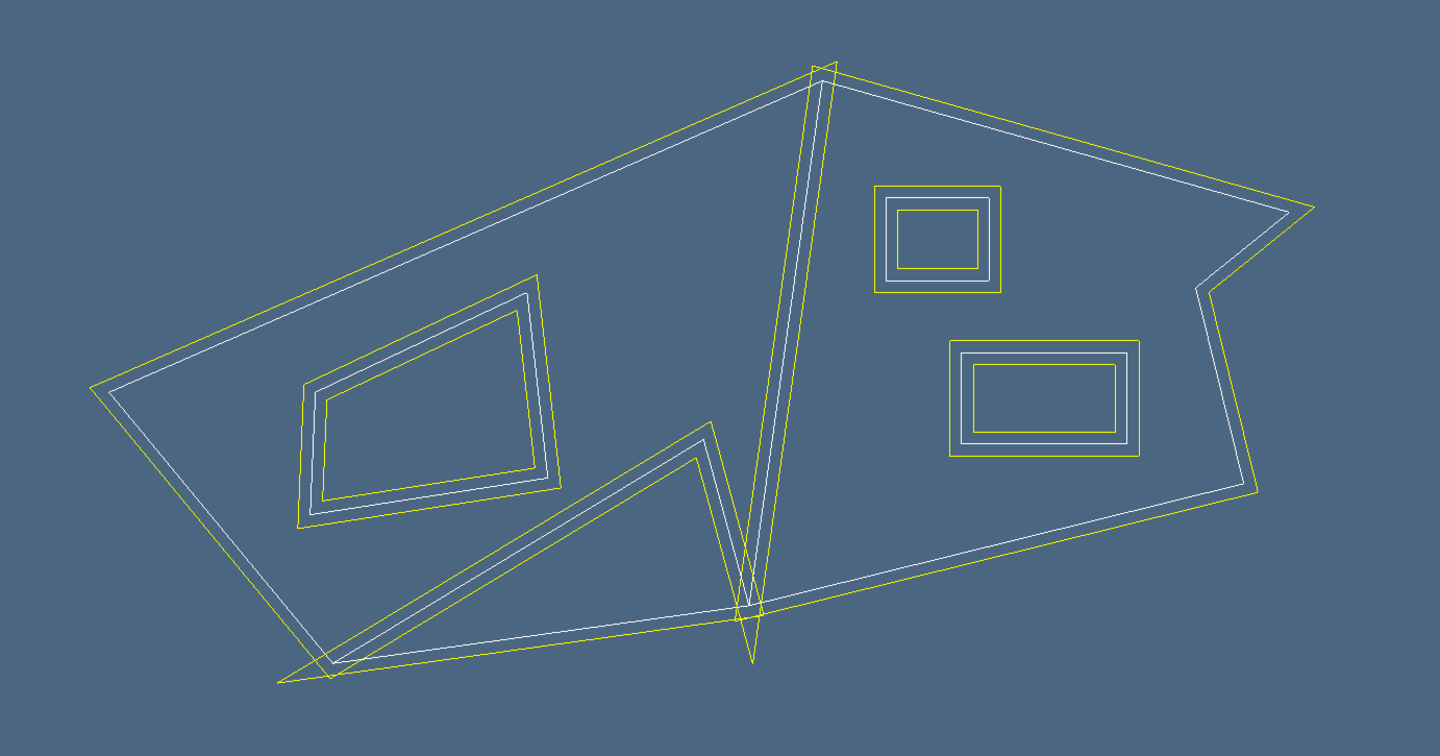
\includegraphics[width=0.49\linewidth]{images/offset2} 
   \caption{(a) the input 2-complex with general LAR cells; (b) drawing of the offset edges (in yellow) generated by \texttt{larOffset2D}.}
   \label{fig:offset}
\end{figure}

\subsection{Extraction of 3-cells from a 2-skeleton embedded in 3D}
Need to characterize the two vertices of zero edge as "last" of previous edge in the chain,
and "first" of following edge in the chain. Therefore the zero edge is oriented as from "last" to "first" and consequently, is "positive" iff  "first" $>$ "last".

It is sufficient to characterize the "first" vertex of the edge following the zero edge. This one is the "last" of zero edge. the other vertex of zero edge is its "first". Zero edge is "positive" iff last(zero) $>$ first(zero).


\paragraph{Choose the next face on ordered coboundary of edge}
Choose the "next" face $g_i$  on "ordered" coboundary of edge


%-------------------------------------------------------------------------------
@D Choose the next face on ordered coboundary of edge
@{""" Choose the next face on ordered coboundary of edge """
def adjFace(boundaryOperator,EV,EF_angle,faceChainOrientation):
    def adjFace0(edge,orientation):
        if orientation > 0:  edgeLoop = REVERSE(EF_angle[edge])
        elif orientation < 0:  edgeLoop = EF_angle[edge]
        edgeLoop = edgeLoop + [edgeLoop[0]]  # all positive indices
        
        candidates = set([f for f,_ in faceChainOrientation]).intersection(edgeLoop)
        if candidates != set([]):
            pivotFace = candidates.pop()
            if pivotFace in edgeLoop:
                pivotIndex = edgeLoop.index(pivotFace)
            else:
                pivotIndex = edgeLoop.index(-pivotFace)
            adjacentFace = edgeLoop[pivotIndex+1]
        else: return None
        
        theSign = boundaryOperator[edge,adjacentFace]
        return adjacentFace, -(theSign*orientation)
    return adjFace0
@}
%-------------------------------------------------------------------------------



\paragraph{Choose the start facet in extracting the facet representation of a cell}
%-------------------------------------------------------------------------------
@D Choose the start facet in extracting the facet representation of a cell
@{""" Choose the start facet in extracting the facet representation of a cell """

def chooseStartFace(FV,faceCounter):
    if faceCounter[0,0]==0: return (0,1)
    for f in range(len(FV)):
        if faceCounter[f,0]==1 and faceCounter[f,1]==0: return (f,-1)
        elif faceCounter[f,0]==0 and faceCounter[f,1]==1: return (f,1)
    for f in range(len(FV)):
        if faceCounter[f,0]==0 and faceCounter[f,1]==0: return (f,1)
    if sum(array(faceCounter))==2*len(FV): return (-1,999)
    else: print "ERROR: chooseStartFace"

def chooseStartFace(FV,faceCounter):
    for f in range(len(FV)):
        if faceCounter[f,0]==1 and faceCounter[f,1]==0: return (f,-1)
        elif faceCounter[f,0]==0 and faceCounter[f,1]==1: return (f,1)
    for f in range(len(FV)):
        if faceCounter[f,0]==0 and faceCounter[f,1]==0: return (f,1)
    if sum(array(faceCounter))==2*len(FV): return (-1,999)
    else: return (0,1)
@}
%-------------------------------------------------------------------------------



\paragraph{Extract the signed representation of a basis element}
%-------------------------------------------------------------------------------
@D Extract the signed representation of a basis element
@{""" Extract the signed representation of a basis element """
def signedBasis(boundaryOperator):
    facesByEdges = csc_matrix(boundaryOperator)
    m,n = facesByEdges.shape
    edges,signs = [],[]
    for i in range(n):
        edges += [facesByEdges.indices[facesByEdges.indptr[
                              i]:facesByEdges.indptr[i+1]].tolist()]
        signs += [facesByEdges.data[facesByEdges.indptr[
                              i]:facesByEdges.indptr[i+1]].tolist()]
    return zip(edges,signs)
@}
%-------------------------------------------------------------------------------


\paragraph{Algoritm} 
The algorithm to compute the signed boundary matrix of a 3-complex is given below in pseudocode.

%-------------------------------------------------------------------------------
\begin{algorithm}
\caption{Compute the signed $\partial_3$ matrix of a 3-complex, from 2-skeleton}
\begin{algorithmic}[1]
\Function {larSignedBoundary3}{LarModel}
    \State {$V,FV,EV \leftarrow {}$LarModel}
    \State {$[\partial_2]\equiv[\delta_1]^t  \leftarrow {}$\textsc{larSignedBoundary2}(LarModel)}
    \State {$sort: EV\to FV\to \R^*: e\mapsto \delta_1(e)$ (ordered loops of signed 2-faces)}
    \State {$[\partial_3]\equiv[\delta_2]^t \leftarrow []$  (boundary 2-faces of 3-cells by row)}
    \State {$S = {}$indices\ of\ 2-faces}
    \While {$S \not= \emptyset$ (set of non-traversed 2-faces) } 
        \State {$f \leftarrow \textsc{choose}(S)$ (first 2-face, reversing previous sign)}
        \State $F \leftarrow \{f\}$ (singleton 2-chain)
        \While {$\partial_2(F) \not= \emptyset$} ($F$ non closed)
            \State $E \leftarrow \partial_2(F) $ (1-cycle of signed edges)
            \While {$E \not= \emptyset$}
                \For {each $e \in E$}
                    \State {$f_i \leftarrow next(f)(sort(\delta_1(e)))$}
                    \State {$F \leftarrow F \cup \{f_i\}$}
                    \State {$S \leftarrow S - \{f_i\}$ (non-traversed 2-faces)}
                    \State {$E \leftarrow E - \{e\}$}
                \EndFor
                \State {$E \leftarrow \partial_2(F) $ (new oriented 1-cycle)}
            \EndWhile
        \EndWhile
        \State {$[\partial_3] \leftarrow [\partial_3]+[F]$ (put F in new $[\partial_3]$ column, i.e.~new $[\delta_2]$ row)}
    \EndWhile 
    \State \Return {$[\partial_3]$ (operator's matrix)}
    \EndFunction 
\end{algorithmic}
\end{algorithm}
%-------------------------------------------------------------------------------



\paragraph{Return the signed boundary matrix of a 3-complex}
%-------------------------------------------------------------------------------
@D Return the signed boundary matrix of a 3-complex
@{""" Return the signed boundary matrix of a 3-complex """
import boolean
def larSignedBoundary3((V,FV,EV)):
    model = V,FV,EV
    faceCounter = zeros((len(FV),2),dtype='b')
    CF,m = [],len(FV)
    efOp = larFaces2Edges(V,FV,EV)
    FE = [efOp([k]) for k in range(len(FV))]
    EF_angle, _,_,_ = boolean.faceSlopeOrdering(model,FE)
    nonWorkedFaces,coboundary_2,cellNumber = set(range(m)),[],0
    boundaryOperator = larSignedBoundary2(V,FV,EV)
    FEbasis = signedBasis(boundaryOperator)
    row,col,data = [],[],[]
    longestrow,longestcol,longestdata,longestLength = [],[],[],0
    while True:
        startFace,orientation = chooseStartFace(FV,faceCounter)
        if startFace == -1: break
        nonWorkedFaces = nonWorkedFaces.difference({startFace})
        faceChainOrientation = {(startFace,orientation)}
        vect = csc_matrix((m,1),dtype='b')
        for face,orientation in faceChainOrientation:  
            vect[face] = orientation
        edgeCycleCoords = boundaryOperator * vect
        edgeCycle = coords2chain(edgeCycleCoords)
        while edgeCycle != []:
            look4face = adjFace(boundaryOperator,EV,EF_angle,faceChainOrientation)
            for edge,orientation in edgeCycle:
                outPair = look4face(edge,orientation)
                if outPair != None:
                    adjacentFace,orientation = outPair
                    faceChainOrientation = faceChainOrientation.union(
                        [(adjacentFace,orientation)])
                    nonWorkedFaces = nonWorkedFaces.difference([adjacentFace])
            vect = csc_matrix((m,1),dtype='b')
            for face,orientation in faceChainOrientation:  
                vect[face] = orientation
            edgeCycleCoords = boundaryOperator * vect
            edgeCycle = coords2chain(edgeCycleCoords)
            #if edgeCycle!=[]: VIEW(STRUCT(MKPOLS((V,[EV[e] for e in TRANS(edgeCycle)[0]]))))
        for face,orientation in faceChainOrientation:
            if orientation == 1: faceCounter[face,0]+=1
            elif orientation == -1: faceCounter[face,1]+=1
        #VIEW(STRUCT(MKPOLS((V,[FV[f] for f in TRANS(faceChainOrientation)[0]]))))
        
        lastrow = [face for face,_ in faceChainOrientation]
        lastcol = [cellNumber for face,orientation in faceChainOrientation]
        lastdata = [orientation for _,orientation in faceChainOrientation]
        lastlength = len(lastrow)
                
        if lastlength >= longestLength:
            lastrow,longestrow = longestrow,lastrow
            lastcol,longestcol = longestcol,lastcol
            lastdata,longestdata = longestdata,lastdata
            lastlength,longestLength = longestLength,lastlength
        if lastlength != 0:
            row += lastrow
            col += lastcol
            data += lastdata
            CF += [lastrow]
            cellNumber += 1 
        print "\nfaceCounter =",faceCounter      
    outMatrix = coo_matrix((data, (row,col)), shape=(m,cellNumber),dtype='b')
    signedBoundary = zip(longestrow,longestdata)
    return csr_matrix(outMatrix),CF,signedBoundary
@}
%-------------------------------------------------------------------------------

\paragraph{Return the signed boundary matrix of a 3-complex}
%-------------------------------------------------------------------------------
@D Return the signed boundary matrix of a 3-complex
@{""" Return the signed boundary matrix of a 3-complex """
import boolean
def larSignedBoundary3((V,FV,EV)):
    model = V,FV,EV
    faceCounter = zeros((len(FV),2),dtype='b')
    CF,m = [],len(FV)
    efOp = larFaces2Edges(V,FV,EV)
    FE = [efOp([k]) for k in range(len(FV))]
    EF_angle, _,_,_ = boolean.faceSlopeOrdering(model,FE)
    nonWorkedFaces,coboundary_2,cellNumber = set(range(m)),[],0
    boundaryOperator = larSignedBoundary2(V,FV,EV)
    FEbasis = signedBasis(boundaryOperator)
    row,col,data = [],[],[]
    while True:
        startFace,orientation = chooseStartFace(FV,faceCounter)
        if startFace == -1: break
        nonWorkedFaces = nonWorkedFaces.difference({startFace})
        faceChainOrientation = {(startFace,orientation)}
        vect = csc_matrix((m,1),dtype='b')
        for face,orientation in faceChainOrientation:  
            vect[face] = orientation
        edgeCycleCoords = boundaryOperator * vect
        edgeCycle = coords2chain(edgeCycleCoords)
        while edgeCycle != []:
            look4face = adjFace(boundaryOperator,EV,EF_angle,faceChainOrientation)
            for edge,orientation in edgeCycle:
                outPair = look4face(edge,orientation)
                if outPair != None:
                    adjacentFace,orientation = outPair
                    faceChainOrientation = faceChainOrientation.union(
                        [(adjacentFace,orientation)])
                    nonWorkedFaces = nonWorkedFaces.difference([adjacentFace])
            vect = csc_matrix((m,1),dtype='b')
            for face,orientation in faceChainOrientation:  
                vect[face] = orientation
            edgeCycleCoords = boundaryOperator * vect
            edgeCycle = coords2chain(edgeCycleCoords)
            #if edgeCycle!=[]: VIEW(STRUCT(MKPOLS((V,[EV[e] for e in TRANS(edgeCycle)[0]]))))
        row += [face for face,_ in faceChainOrientation]
        col += [cellNumber for face,orientation in faceChainOrientation]
        data += [orientation for _,orientation in faceChainOrientation]
        cellNumber += 1
        
        for face,orientation in faceChainOrientation:
          if orientation == 1: faceCounter[face,0]+=1
          elif orientation == -1: faceCounter[face,1]+=1
        print "faceChainOrientation =",faceChainOrientation   
        print "faceCounter =",faceCounter   
          
        CF += [[face for face,_ in faceChainOrientation]]
        print "CF =",CF
        print "\nfaceCounter =",faceCounter      
    outMatrix = coo_matrix((data, (row,col)), shape=(m,cellNumber),dtype='b')
    return csr_matrix(outMatrix),CF,faceCounter
@}
%-------------------------------------------------------------------------------


\begin{figure}[htbp] %  figure placement: here, top, bottom, or page
   \centering
   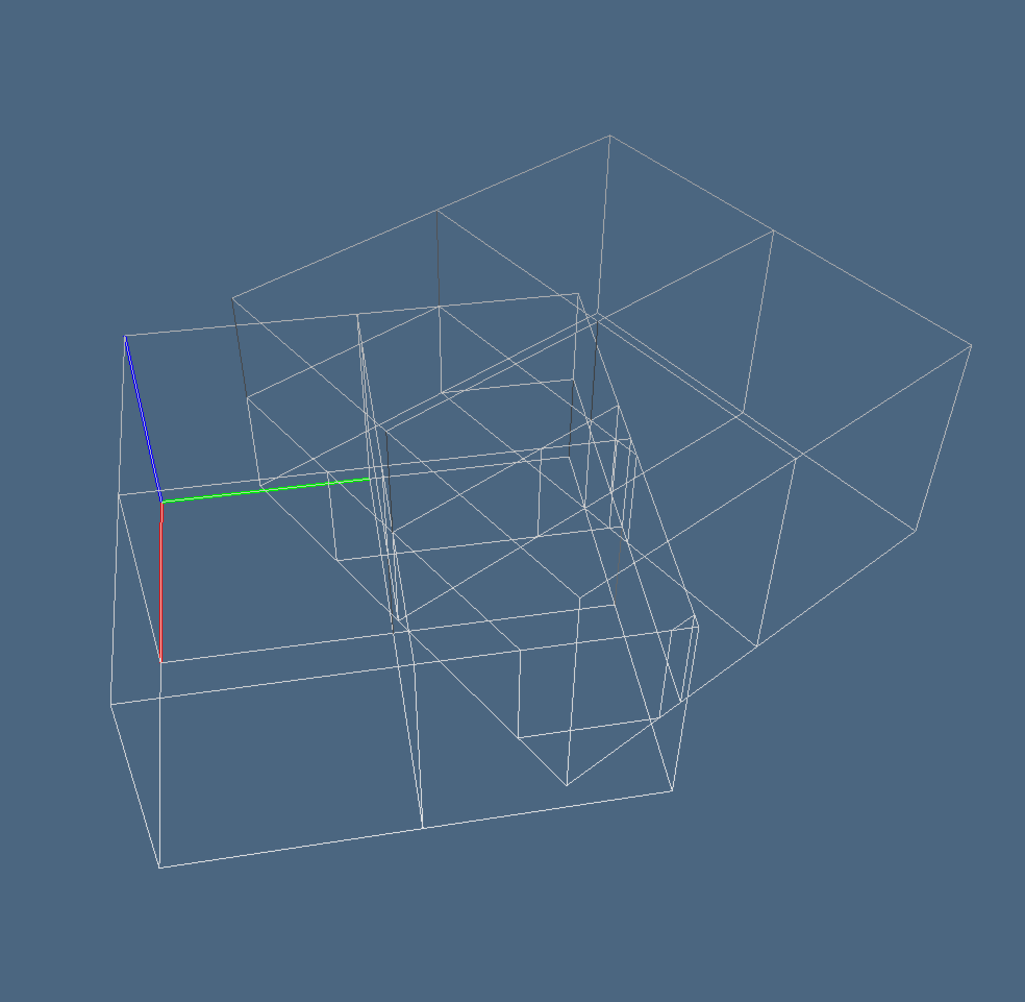
\includegraphics[width=0.295\linewidth]{images/signbound-0} 
   %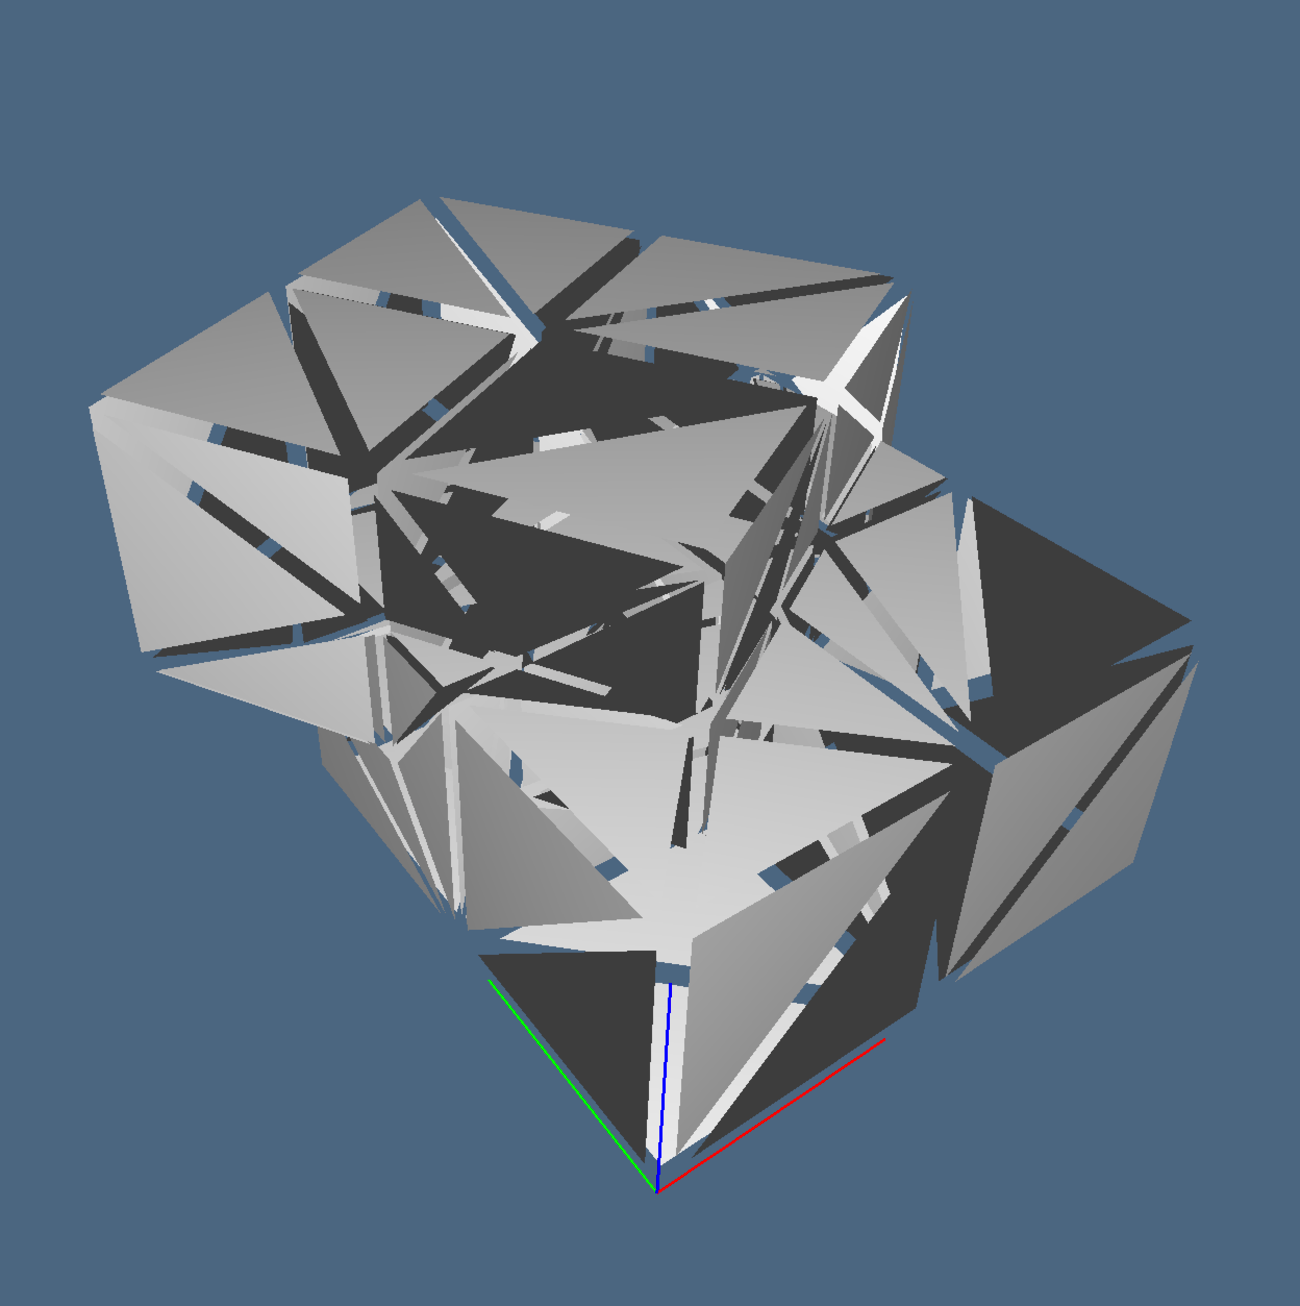
\includegraphics[width=0.245\linewidth]{images/signbound-2} 
   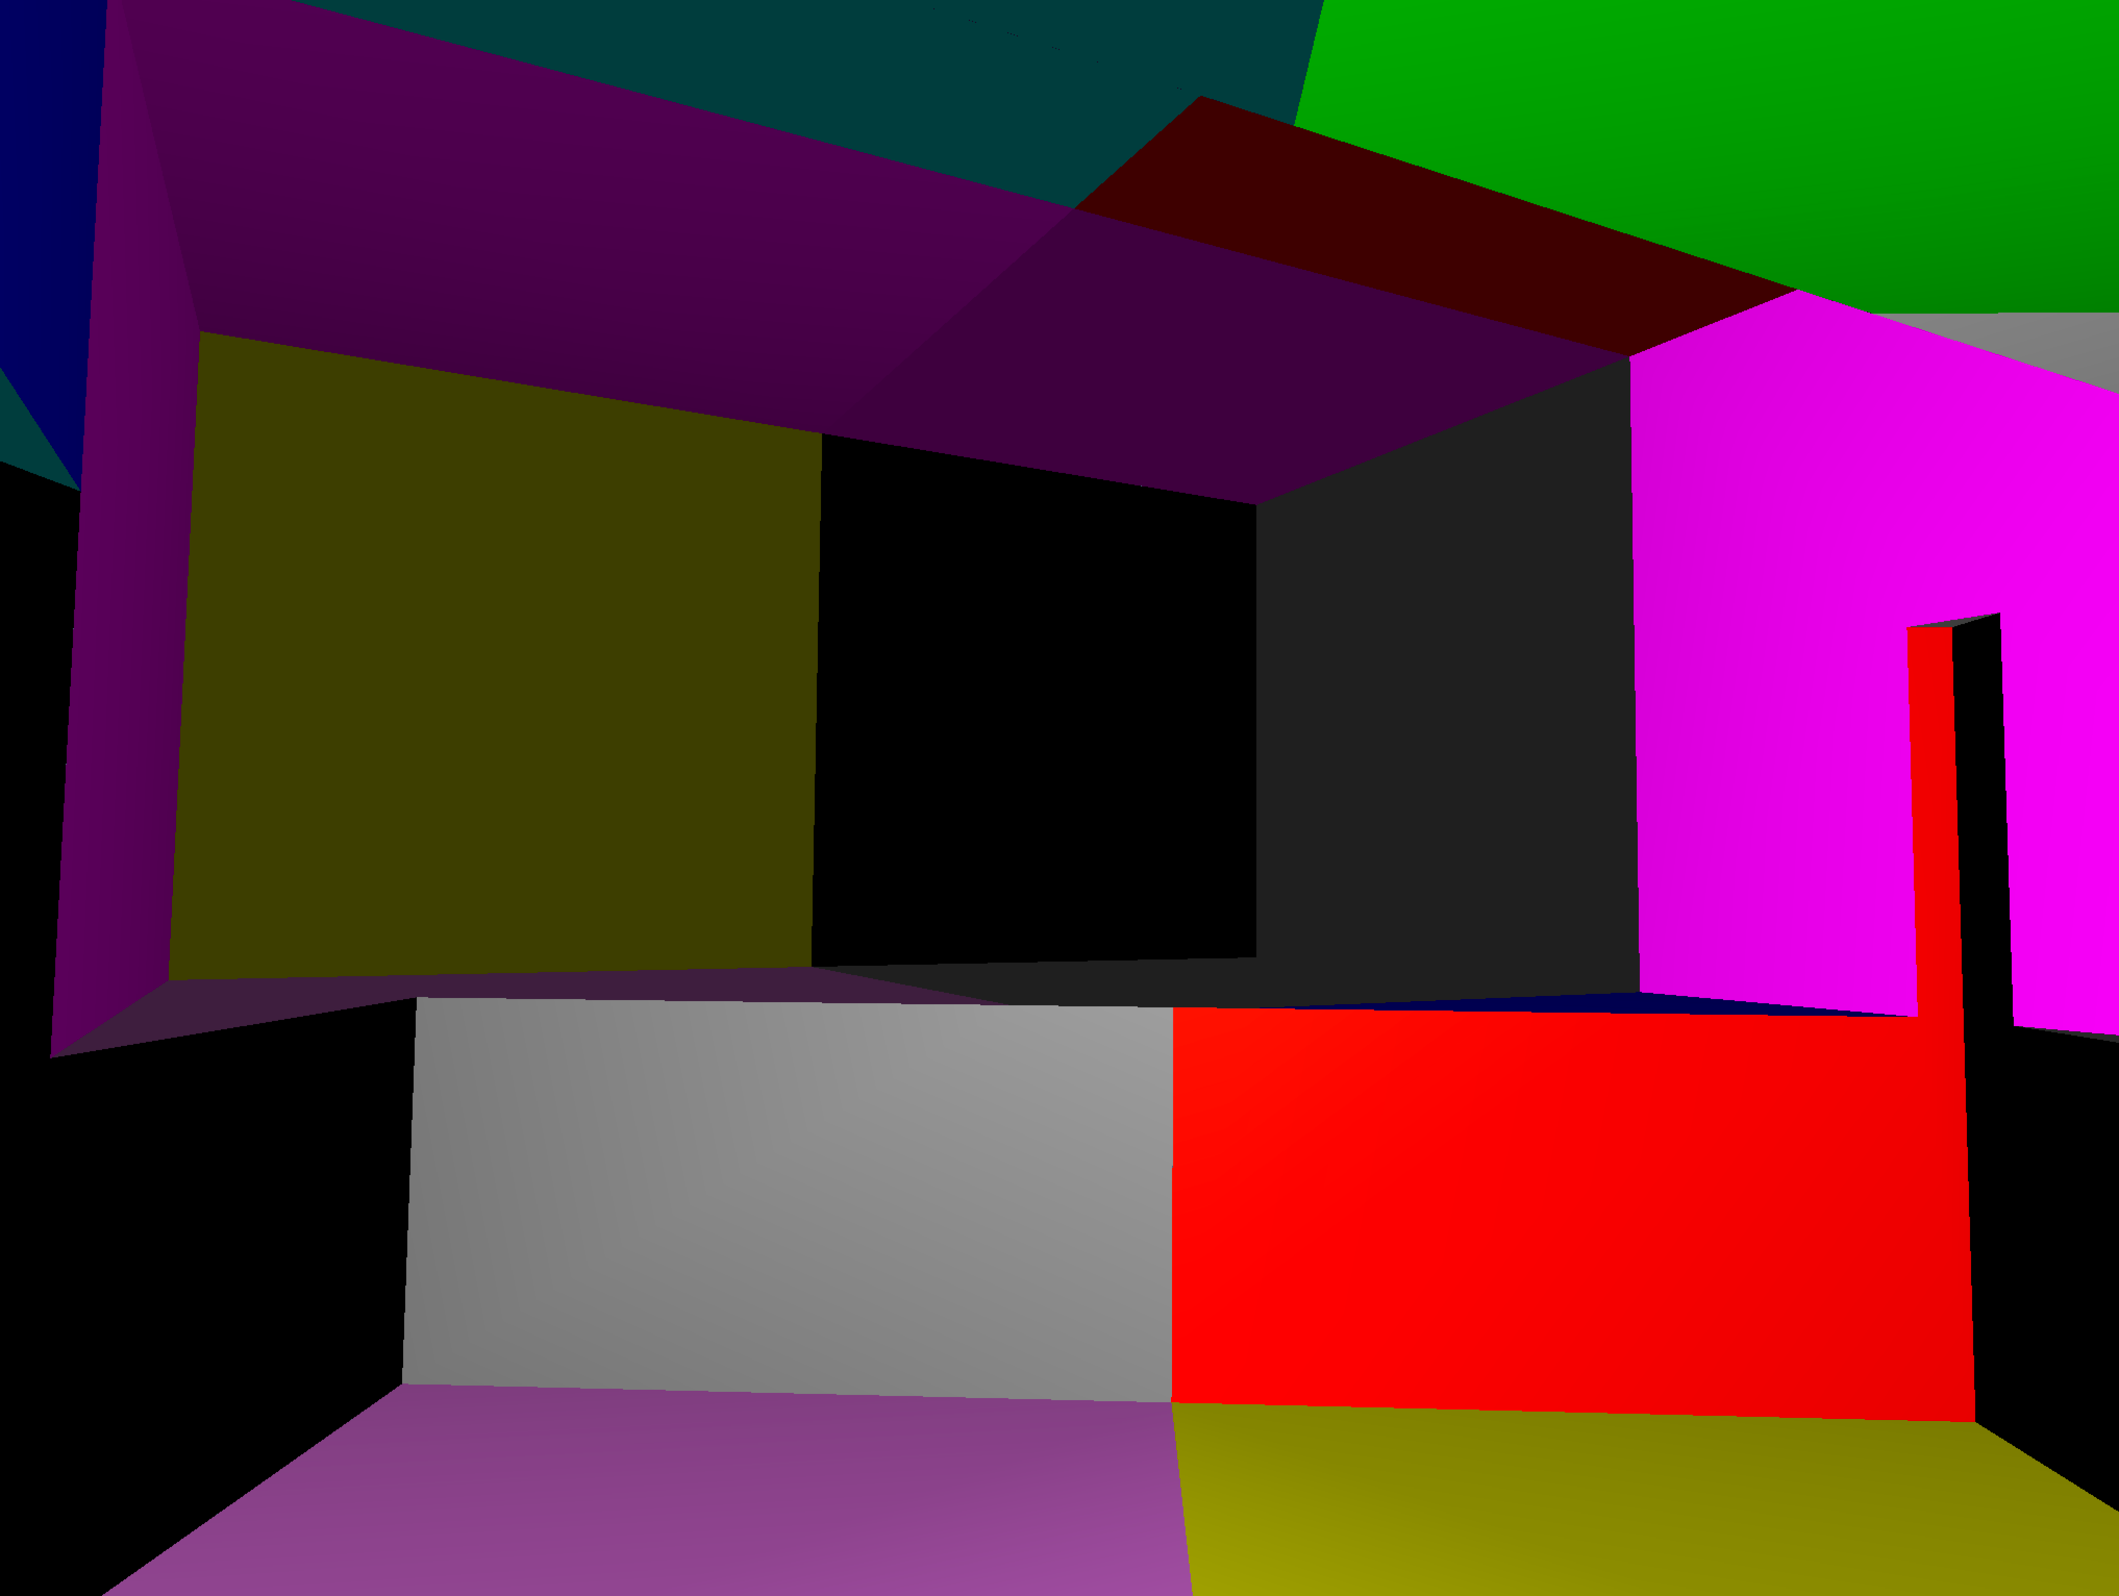
\includegraphics[width=0.385\linewidth]{images/signbound-3} 
   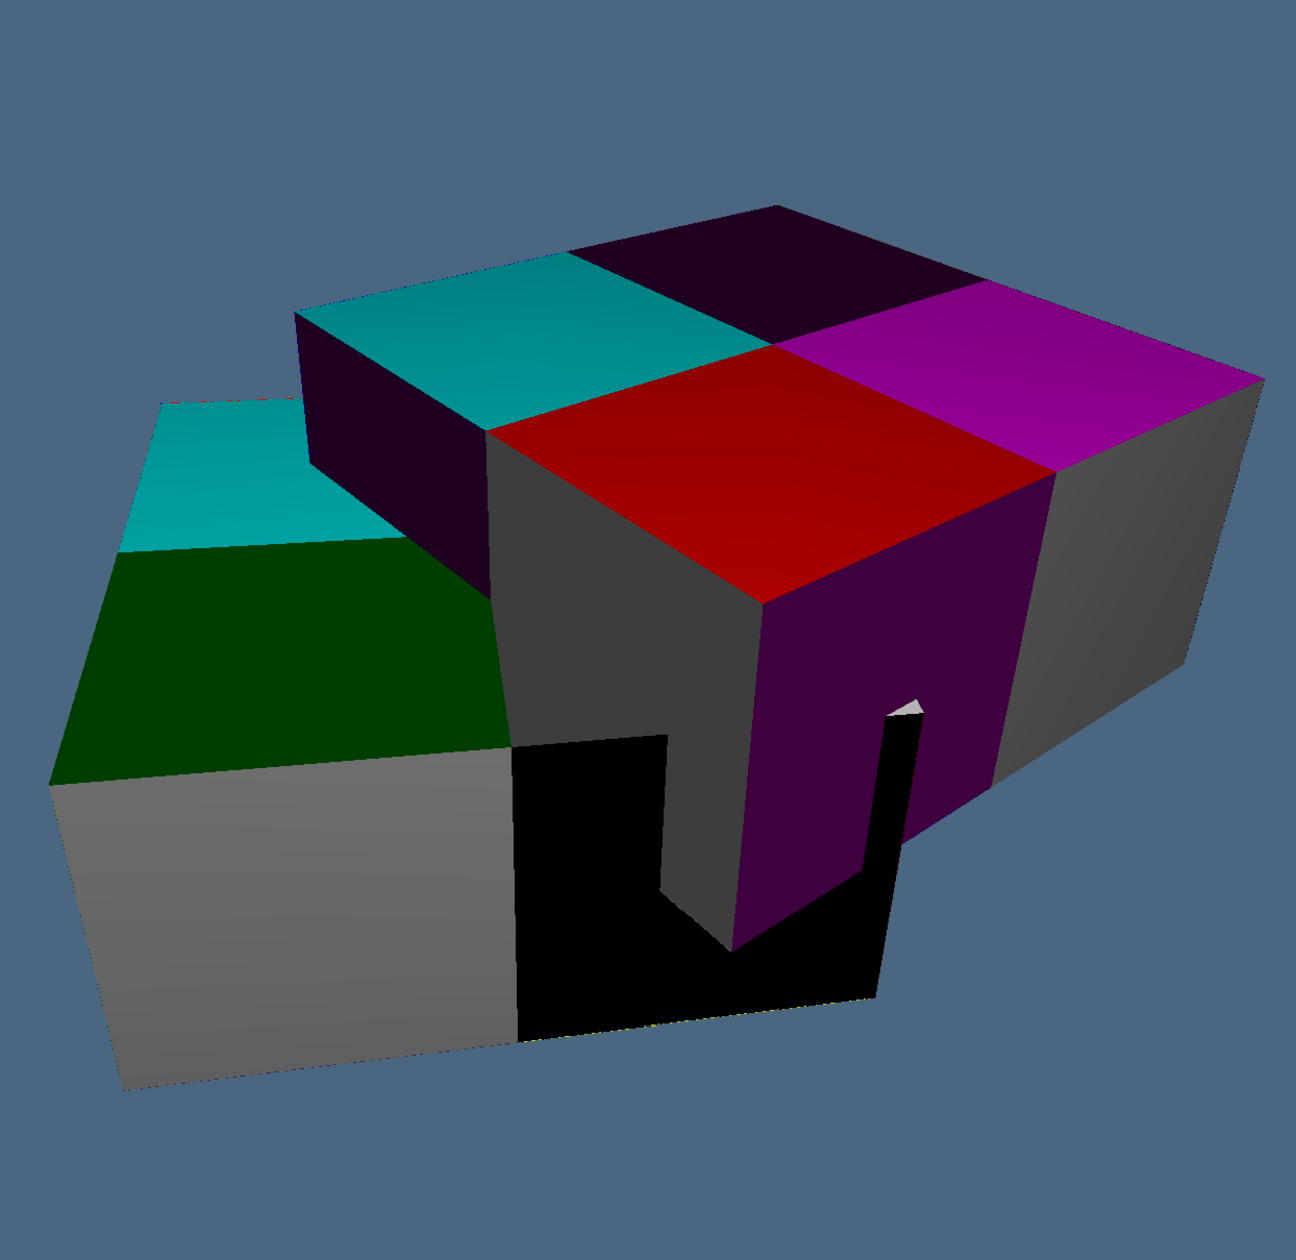
\includegraphics[width=0.30\linewidth]{images/signbound-4} 
   \caption{Arrangment of 3-complexes: (a) 1-skeleton of the fragmented (union) 3-complex; (b) view from the interior of the boundary 2-complex; (c) view from the exterior of the 3-complex.
   Notice that the colour patches correspond to the chain of 2-faces of the boundary of 3-complex.
   }
   \label{fig:signbound}
\end{figure}

\paragraph{Test the signed boundary matrix of a 3-complex}
%-------------------------------------------------------------------------------
@D Test the signed boundary matrix of a 3-complex
@{""" Test the signed boundary matrix of a 3-complex """
if __name__=="__main__":

    V,[VV,EV,FV,CV] = larCuboids([2,2,1],True)
    cubeGrid = Struct([(V,FV,EV)],"cubeGrid")
    cubeGrids = Struct(2*[cubeGrid,t(.5,.5,.5),r(0,0,PI/6)])

    V,FV,EV = struct2Marshal(cubeGrids)
    VIEW(EXPLODE(1.2,1.2,1.2)(BREP((V,FV,EV),color=False) ))
@}
%-------------------------------------------------------------------------------


\subsection{Examples}

\paragraph{A 3-cell with several holes}
%-------------------------------------------------------------------------------
@O test/py/boundary/test12.py
@{""" testing boundary operators (correct result) """
from larlib import *

V,[VV,EV,FV,CV] = larCuboids([1,1,1],True)
cell = (V,FV,EV)
cubeGrid =  Struct([Struct([ s(10,10,1),cell ])] + 3*[t(0,2,0), Struct(3*[ t(1.5,0,0), cell] )] ,"cubeGrid")
VIEW(STRUCT(MKPOLS(struct2lar(cubeGrid))))

V,FV,EV = struct2Marshal(cubeGrid)
csrmat,CF,faceCounter = larSignedBoundary3((V,FV,EV))
print csrmat.todense()
@}
%-------------------------------------------------------------------------------



\section{Exporting}
%===============================================================================


%-------------------------------------------------------------------------------
@O larlib/larlib/boundary.py
@{""" boundary operators """
from larlib import *
@< convex-cells boundary operator @>
@< path-connected-cells boundary operator @>
@< From cells and facets to boundary cells @>
@< Marshalling a structure to a LAR cellular model @>
@< Compute the signed 2-boundary matrix @>
@< Compute any signed 1-boundary chain @>
@< Offset of 2-faces of a 2D complex @>
@< Boundary of a 3-complex @>
@< Query from 3-chain to incident 2-chain @>
@< Query from 3-chain to incident 1-chain @>
@< Query from 2-chain to incident 1-chain @>
@< kfaces-to-kfaces relations @>
@< Transformation from chain coordinates to explicit chain data @>
@< Choose the next face on ordered coboundary of edge @>
@< Choose the start facet in extracting the facet representation of a cell @>
@< Extract the signed representation of a basis element @>
@< Return the signed boundary matrix of a 3-complex @>
@< Test the signed boundary matrix of a 3-complex @>
@}
%-------------------------------------------------------------------------------


\section{Testing}

\subsection{Non-oriented operators}

\paragraph{Correct boundary extraction example}

The \texttt{larBoundary()} operator is applied here to a cellular 2-complex of convex cells, producing correct result. It is worth noting that the operator is dimension-independent, and must be appliad to the \emph{pair} of compressed characteristic matrices $M_d$ and $M_{d-1}$, that --- in list format --- we call either \texttt{CV,FV} or  \texttt{FV,EV}, depending on the dimension (either 3 or 2) of the embedding space.

%-------------------------------------------------------------------------------
@O test/py/boundary/test01.py
@{""" testing boundary operators (correct result) """
from larlib import *

filename = "test/svg/inters/boundarytest0.svg"
lines = svg2lines(filename)
VIEW(STRUCT(AA(POLYLINE)(lines)))
    
V,FV,EV,polygons = larFromLines(lines)
VV = AA(LIST)(range(len(V)))
submodel = STRUCT(MKPOLS((V,EV)))
VIEW(larModelNumbering(1,1,1)(V,[VV,EV,FV],submodel,0.2))
VIEW(EXPLODE(1.2,1.2,1.2)(MKPOLS((V,[EV[e] for e in boundaryCells(FV,EV)],))))
VIEW(EXPLODE(1.2,1.2,1.2)(MKTRIANGLES((V,FV,EV))))

boundaryOp = larUnsignedBoundary2(FV,EV,VV)

for k in range(1,len(FV)+1):
    faceChain = k*[1]
    BF = chain2BoundaryChain(boundaryOp)(faceChain)
    VIEW(STRUCT(MKPOLS((V,[EV[e] for e in BF]))))
@}
%-------------------------------------------------------------------------------

\paragraph{Wrong boundary extraction example}

The \texttt{larBoundary()} operator, applied  to a cellular 2-complex wih some non-convex cells, produces incorrect results. In such cases a correct result may be produced only by chance (sometimes this happens). So, be careful to use it only when the precondition (of cell convexity) is everywhere verified. In order to get always a correct result, use the \texttt{larUnsignedBoundary2} operator.

%-------------------------------------------------------------------------------
@O test/py/boundary/test02.py
@{""" testing boundary operators (wrong result) """
from larlib import *

filename = "test/svg/inters/boundarytest3.svg" # KO (MKTRIANGLES) with boundarytest3 !!!
#filename = "test/svg/inters/boundarytest4.svg"
lines = svg2lines(filename)
VIEW(STRUCT(AA(POLYLINE)(lines)))
    
V,FV,EV,polygons = larFromLines(lines)
VV = AA(LIST)(range(len(V)))
submodel = STRUCT(MKPOLS((V,EV)))
VIEW(larModelNumbering(1,1,1)(V,[VV,EV,FV],submodel,0.2))

boundaryOp = larUnsignedBoundary2(FV,EV,VV)  # <<======  NB
#boundaryOp = larBoundary(FV,EV)  # <<======  NB
BF = chain2BoundaryChain(boundaryOp)([1]*len(FV))

VIEW(EXPLODE(1.2,1.2,1.2)(MKPOLS((V,[EV[e] for e in BF])))) 
VIEW(EXPLODE(1.2,1.2,1.2)(MKTRIANGLES((V,FV,EV),color=True))) 
VIEW(SKEL_1(EXPLODE(1.2,1.2,1.2)(MKTRIANGLES((V,FV,EV))))) 
"""
for k in range(1,len(FV)+1):
    faceChain = k*[1]
    boundaryChain = chain2BoundaryChain(boundaryOp)(faceChain)
    VIEW(STRUCT(MKPOLS((V,[EV[e] for e in boundaryChain]))))
"""
@}
%-------------------------------------------------------------------------------

\begin{figure}[htbp] %  figure placement: here, top, bottom, or page
   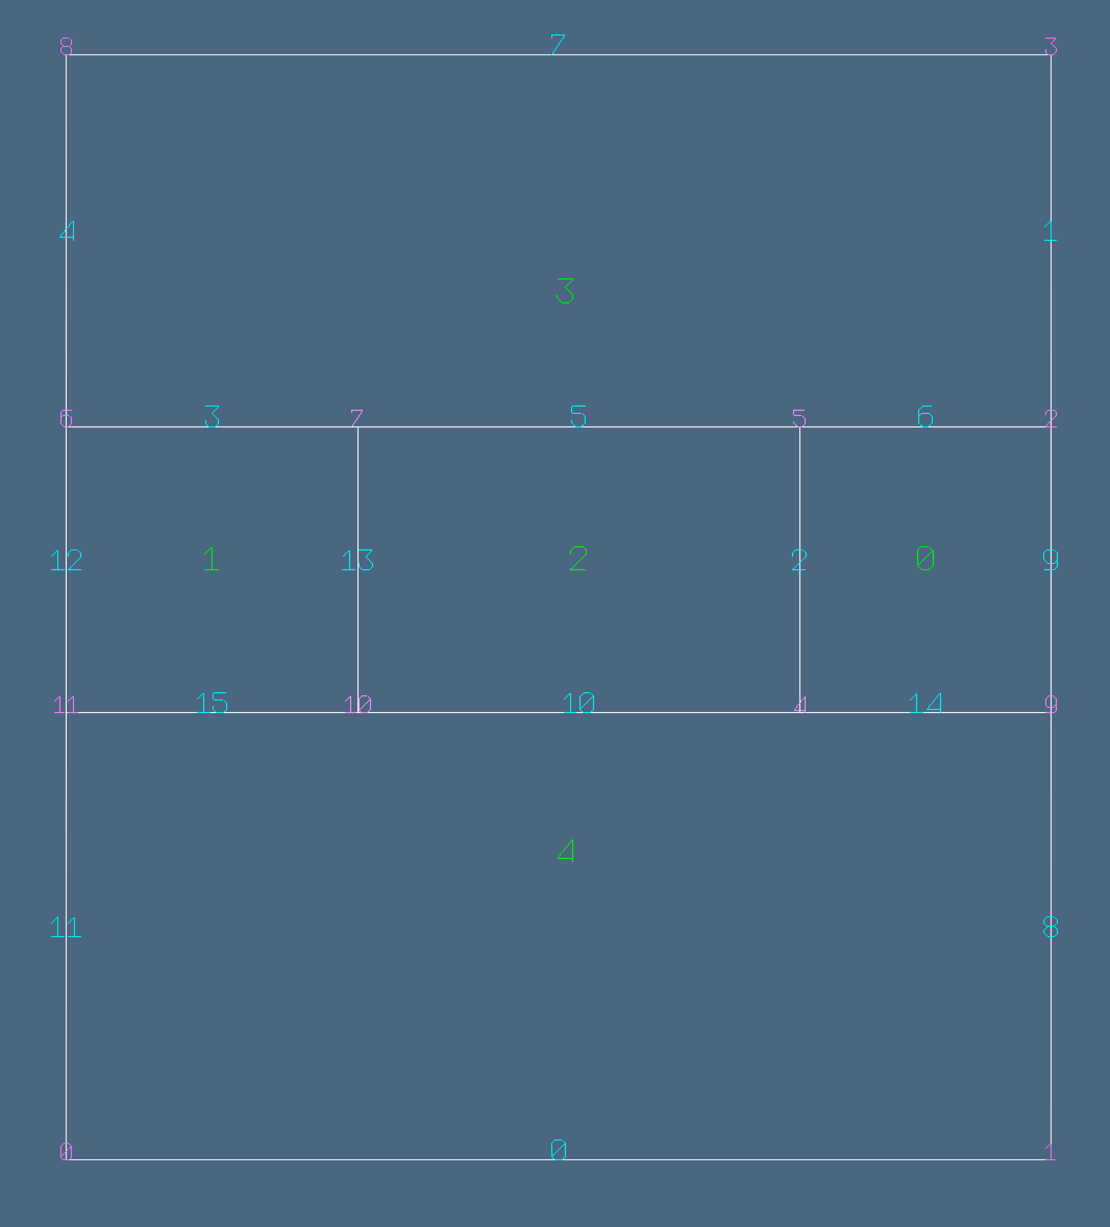
\includegraphics[height=0.245\linewidth,width=0.245\linewidth]{images/boundary-test01-2} 
   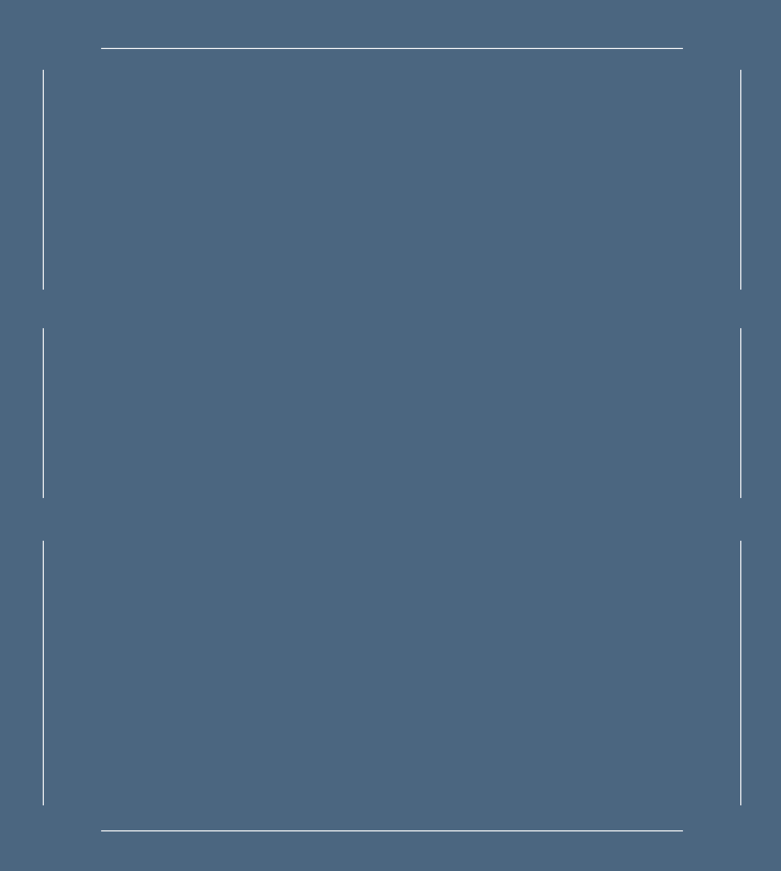
\includegraphics[height=0.245\linewidth,width=0.245\linewidth]{images/boundary-test01-3} 
   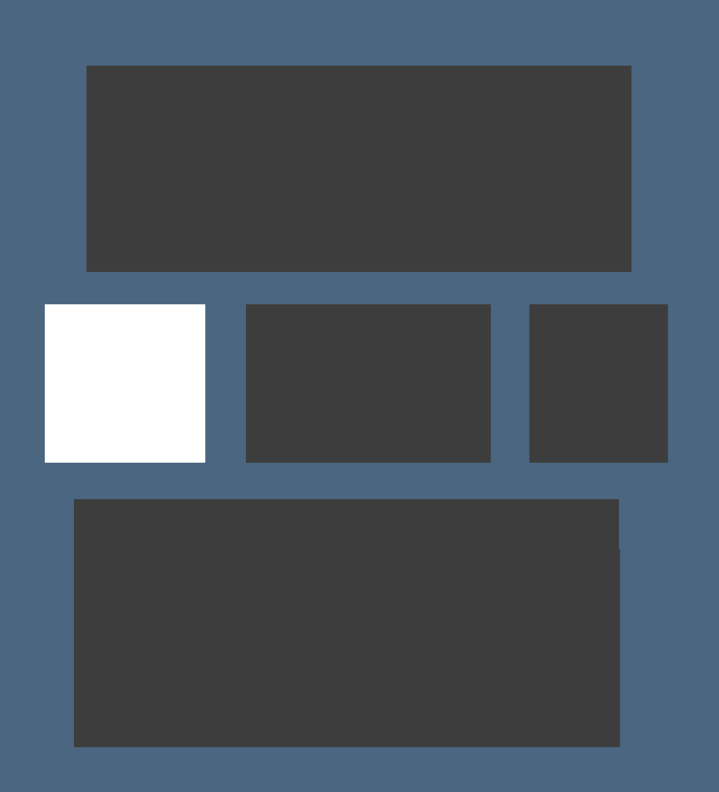
\includegraphics[height=0.245\linewidth,width=0.245\linewidth]{images/boundary-test01-4} 
   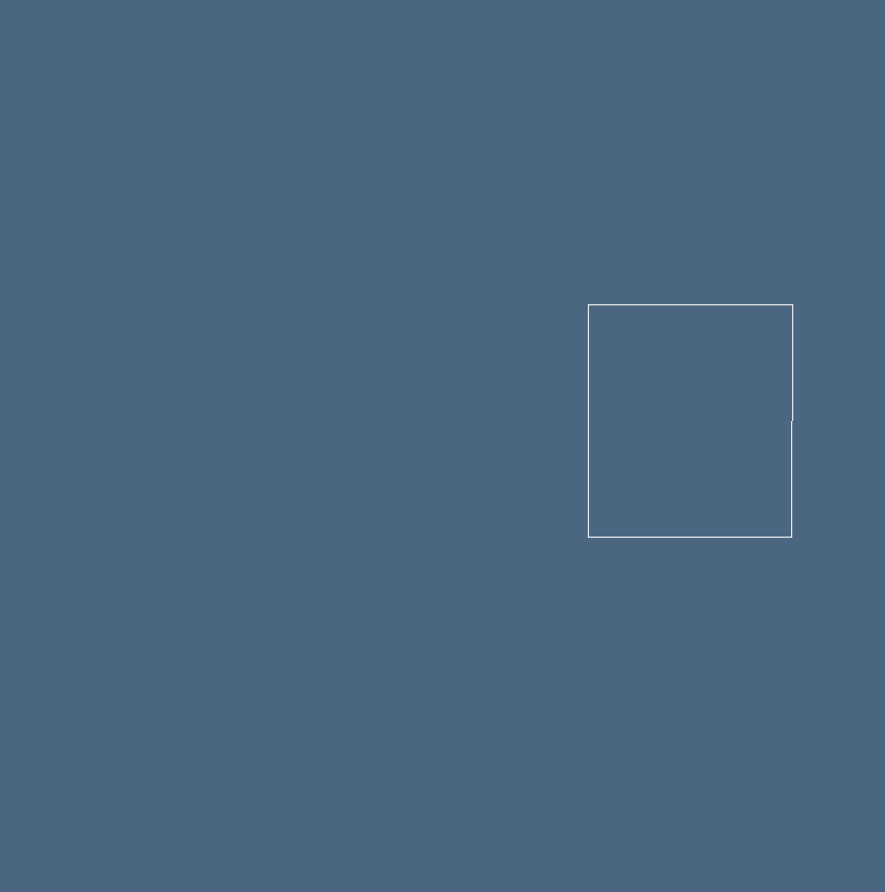
\includegraphics[height=0.245\linewidth,width=0.245\linewidth]{images/boundary-test01-5} 

   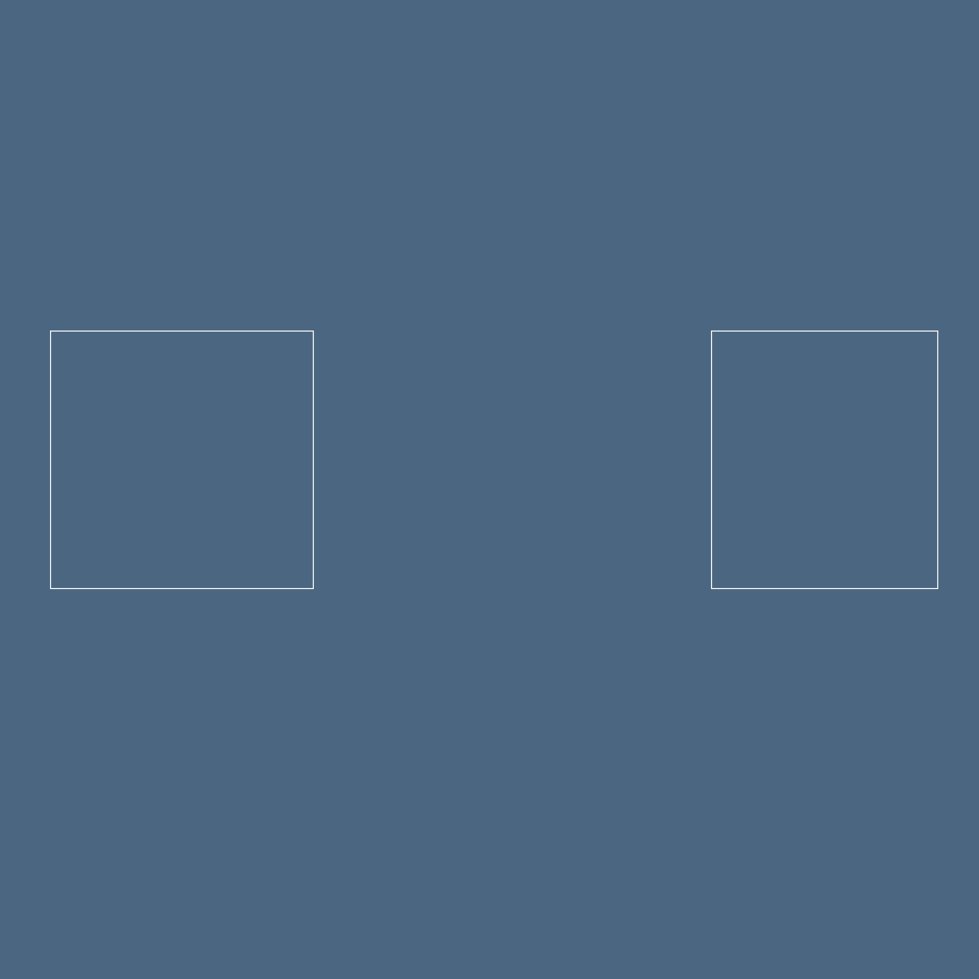
\includegraphics[height=0.245\linewidth,width=0.245\linewidth]{images/boundary-test01-6} 
   
\includegraphics[height=0.245\linewidth,width=0.245\linewidth]{images/boundary-test01-7} 
   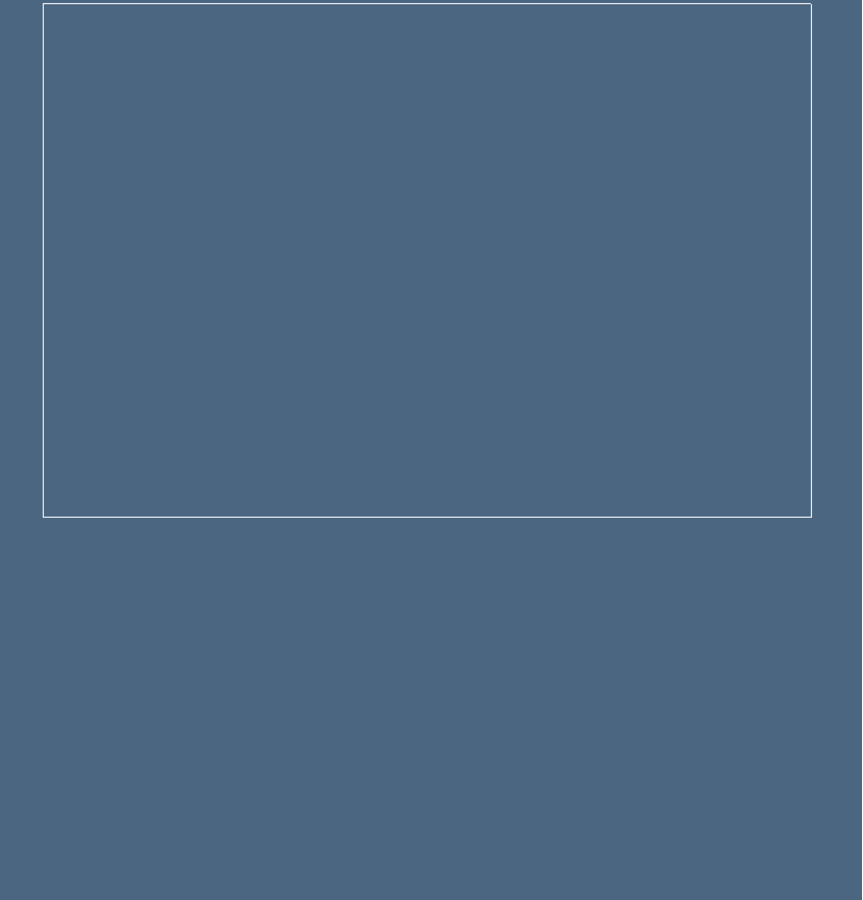
\includegraphics[height=0.245\linewidth,width=0.245\linewidth]{images/boundary-test01-8} 
   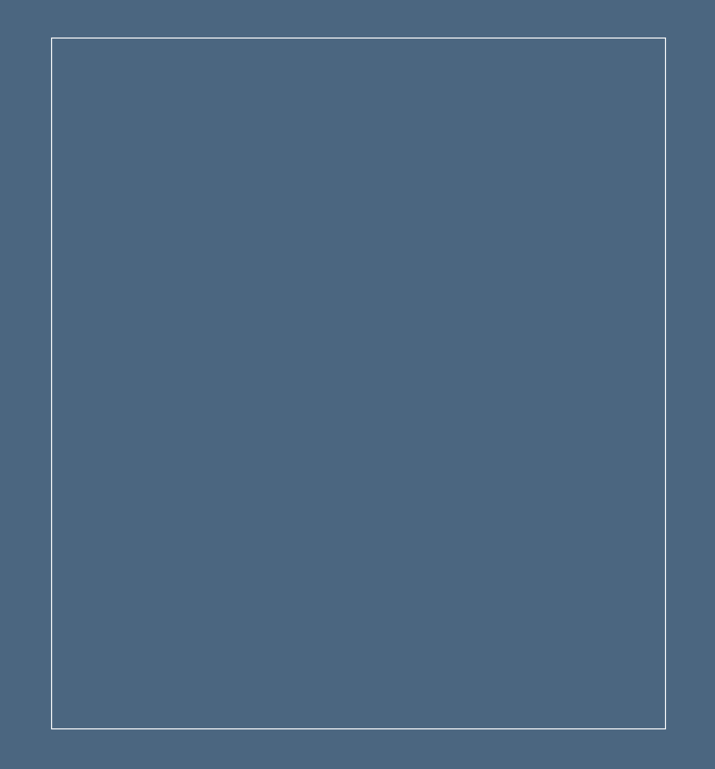
\includegraphics[height=0.245\linewidth,width=0.245\linewidth]{images/boundary-test01-9} 
   \caption{Convex-cell 2-complex. (a) Indexing of 0-,1-,and 2-cells; (b) exploded 2-boundary cells; (c) exploded 2-cells; (d) boundary of a singleton 2-chain; (e--h) boundaries of some 2-chains.}
   \label{fig:example}
\end{figure}

\paragraph{Example}
Comparison of two implementations of the $\partial$ operator. Notice the difference between the penultimate rows. In particular, the penultimate row of the matrix generated by \texttt{larBoundary(FV,EV)} is plain wrong. It means that the edge $e_{10}$ is shared by all the (three) 2-cells of the complex. Conversely, it is well known that, for a solid complex, i.e.~a $d$-complex embedded in $\mathbb{E}^d$, every $(d-1)$-facet may be shared by no more than 2 $d$-cells. The resulting boundary of the total chain $[f_0, f_1, f_2]$ codified in coordinates as $[1,1,1]$, and shown in Figure~\ref{fig:boundary-test02}d, is sonsequently incorrect.
\\[3mm]

%-------------------------------------------------------------------------------
{\scriptsize
\begin{minipage}[c]{0.5\linewidth}
\centering
\begin{verbatim}
In [1]: larBoundary(FV,EV).todense()
Out[1]: 
matrix([[0, 1, 0],
        [0, 0, 1],
        [1, 0, 1],
        [1, 0, 1],
        [0, 1, 1],
        [0, 1, 0],
        [1, 0, 1],
        [0, 0, 1],
        [0, 0, 1],
        [0, 1, 0],
        [1, 1, 1],
        [0, 1, 1]])
\end{verbatim}
\end{minipage}
\begin{minipage}[c]{0.5\linewidth}
\centering
\begin{verbatim}
In [2]: larUnsignedBoundary2(FV,EV,VV).todense()
Out[2]: 
matrix([[0, 1, 0],
        [0, 0, 1],
        [1, 0, 1],
        [1, 0, 1],
        [0, 1, 1],
        [0, 1, 0],
        [1, 0, 1],
        [0, 0, 1],
        [0, 0, 1],
        [0, 1, 0],
        [1, 1, 0],
        [0, 1, 1]])
\end{verbatim}
\end{minipage}}
%-------------------------------------------------------------------------------


\begin{figure}[htbp] %  figure placement: here, top, bottom, or page
   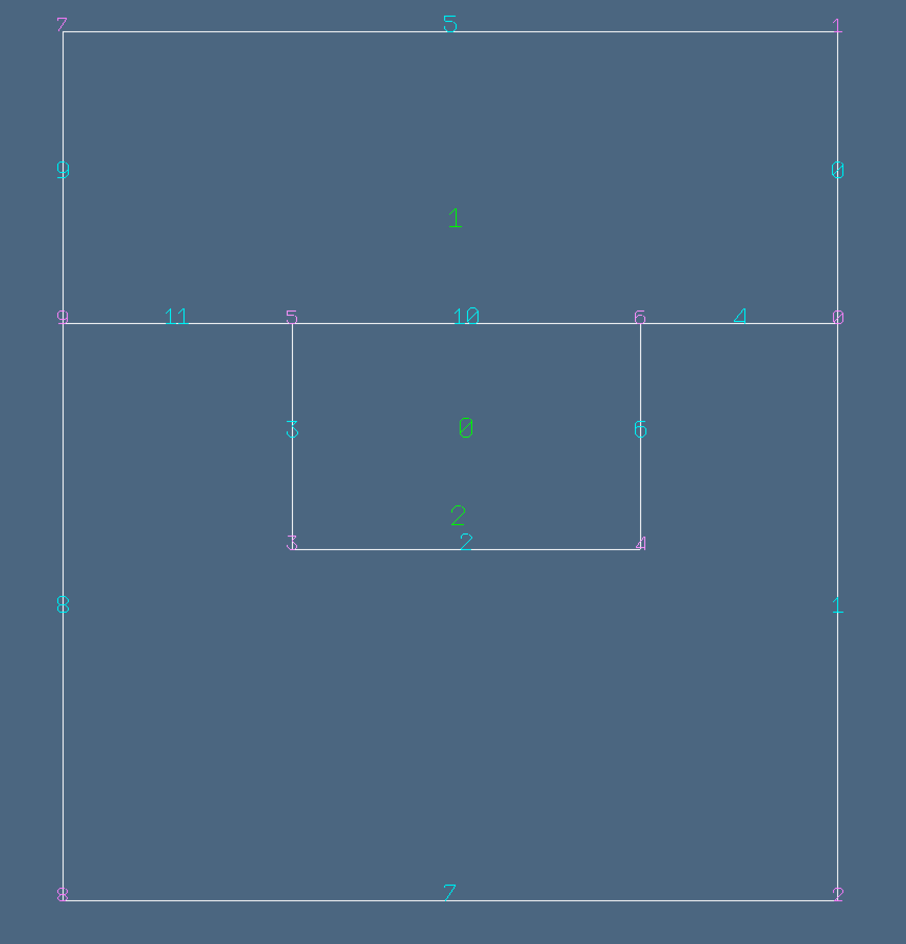
\includegraphics[height=0.245\linewidth,width=0.245\linewidth]{images/boundary-test02-1} 
   
\includegraphics[height=0.245\linewidth,width=0.245\linewidth]{images/boundary-test02-2} 
   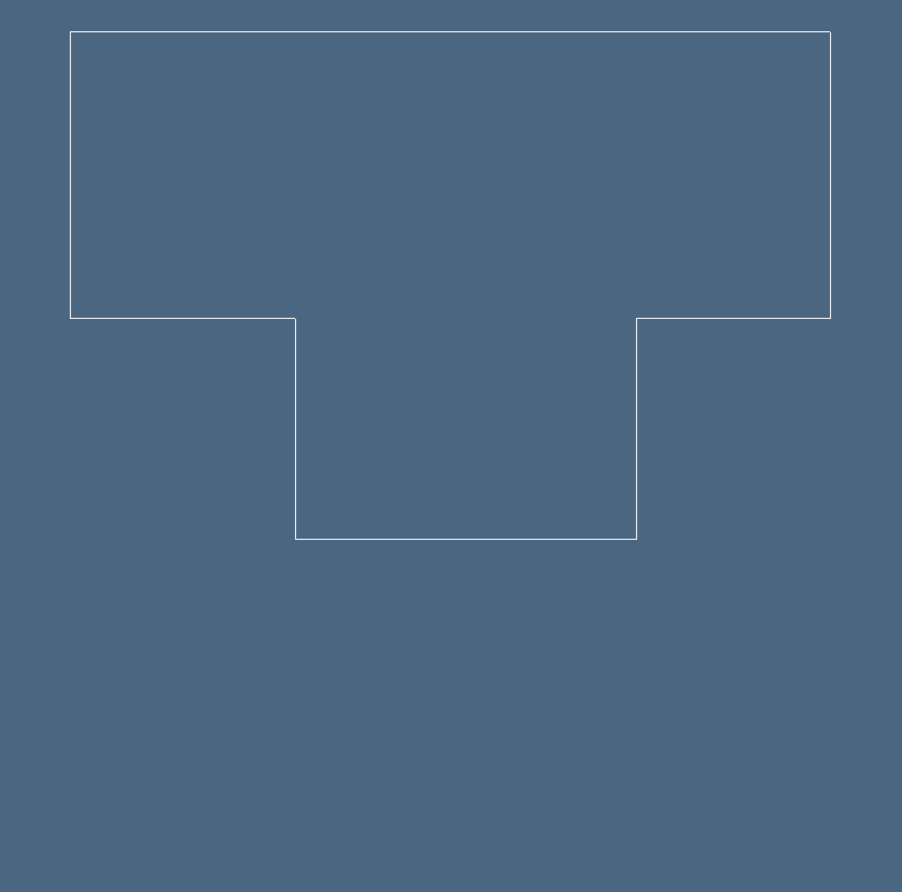
\includegraphics[height=0.245\linewidth,width=0.245\linewidth]{images/boundary-test02-3} 
   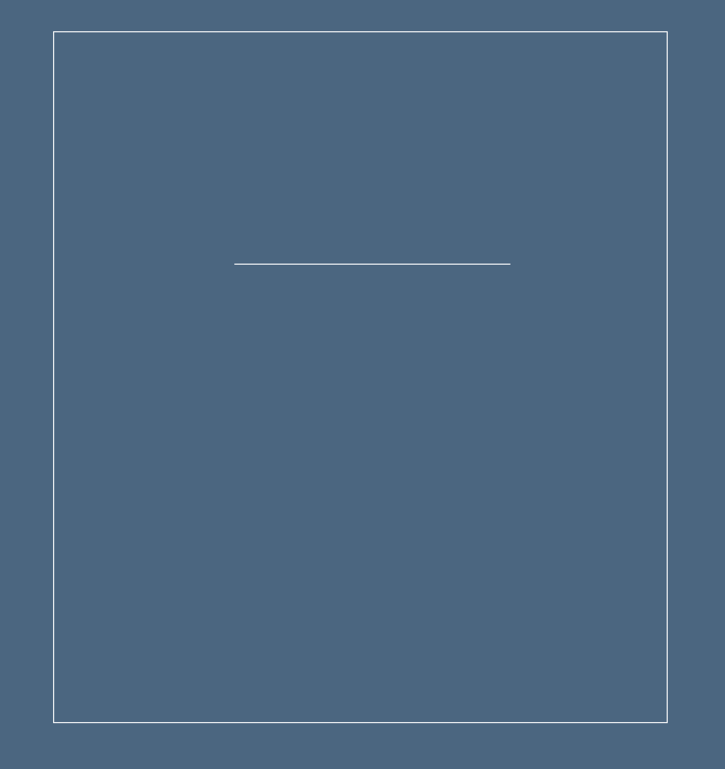
\includegraphics[height=0.245\linewidth,width=0.245\linewidth]{images/boundary-test02-4} 

   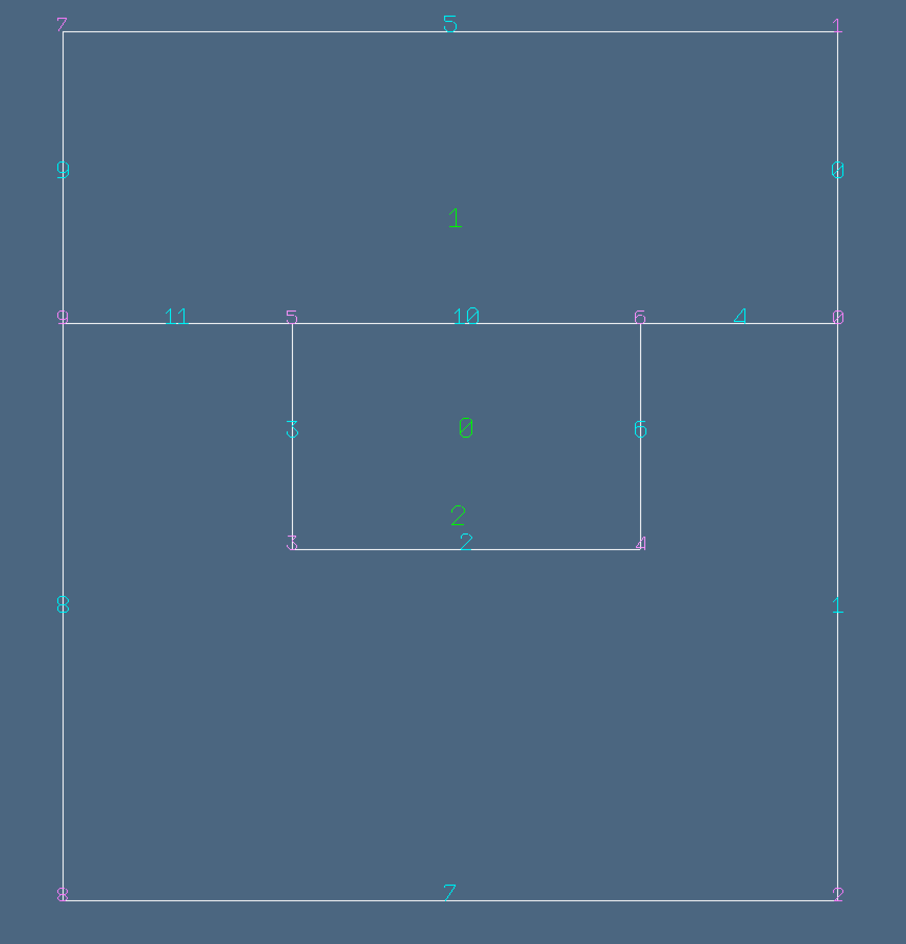
\includegraphics[height=0.245\linewidth,width=0.245\linewidth]{images/boundary-test02-1} 
   
\includegraphics[height=0.245\linewidth,width=0.245\linewidth]{images/boundary-test02-2} 
   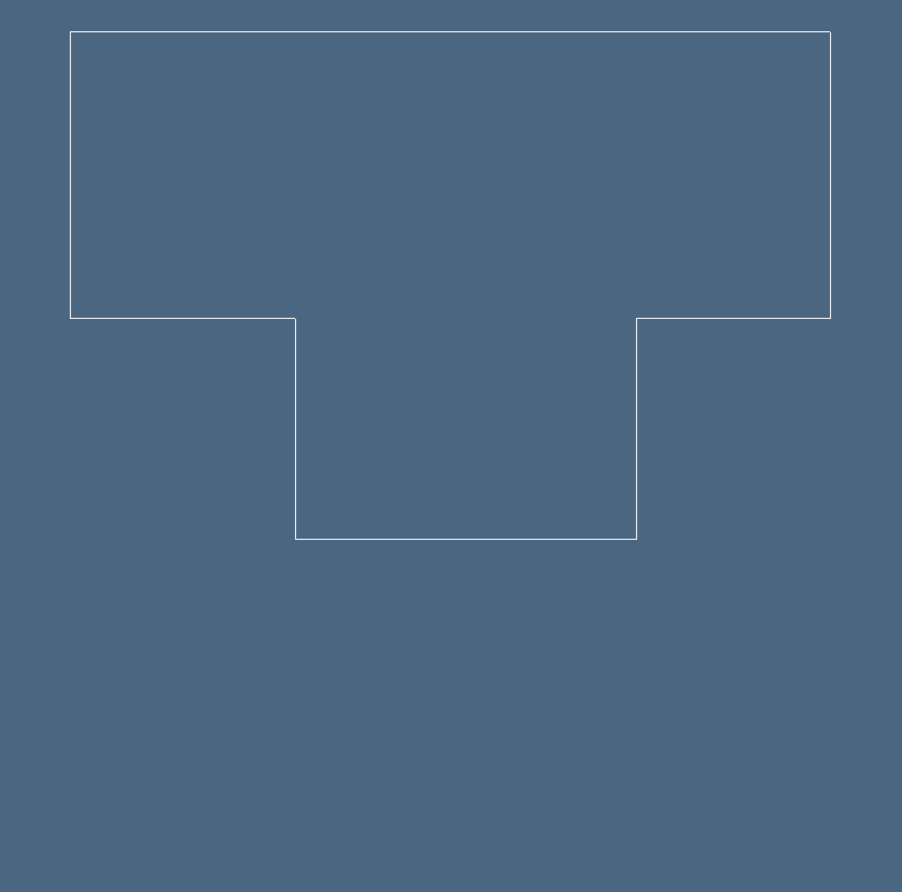
\includegraphics[height=0.245\linewidth,width=0.245\linewidth]{images/boundary-test02-3} 
   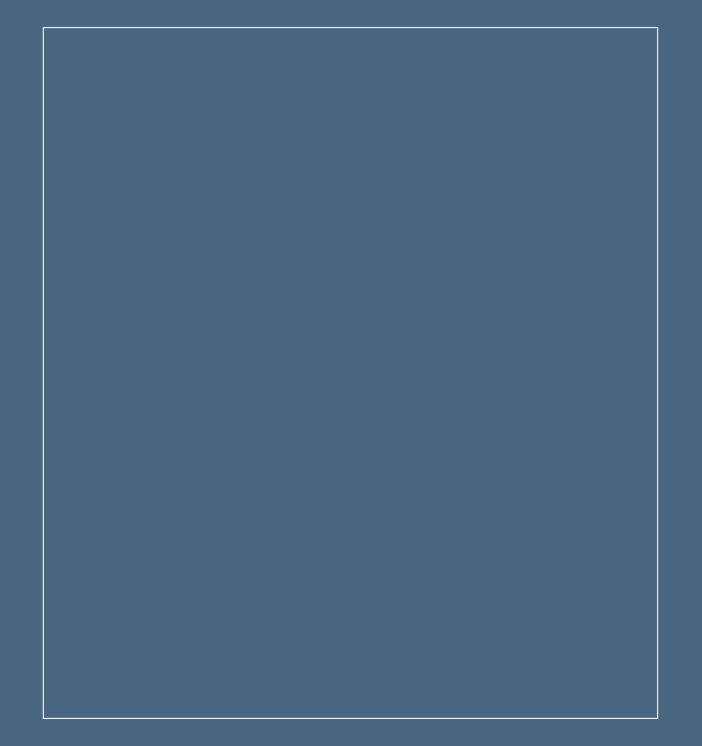
\includegraphics[height=0.245\linewidth,width=0.245\linewidth]{images/boundary-test02-5} 
   \caption{Non-working (i.e.~\emph{wrong}) example with \texttt{boundary}. (a) Indexing of 0-,1-,and 2-cells; (b) boundary of a singleton 2-chain; (c) exploded 2-cells; (d) boundary of a singleton 2-chain. Working (i.e.~\emph{exact}) example using \texttt{larUnsignedBoundary2}: (e--h) as above.}
   \label{fig:boundary-test02}
\end{figure}


\paragraph{3D non-convex LAR cells}
In this example and in the next one we show the boundary computation of LAR models with non-contractible 3- and 2-cells.

%-------------------------------------------------------------------------------
@O test/py/boundary/test03.py
@{""" 3D non-convex LAR cells """
from larlib import *

V = [[0.25,0.25,0.0],[0.25,0.75,0.0],[0.75,0.75,0.0],[0.75,0.25,0.0],[1.0, 0.0,0.0],
[0.0,0.0,0.0],[1.0,1.0,0.0],[0.0,1.0,0.0],[0.25,0.25,1.0],[0.25, 0.25,2.0],[0.25,0.75,
2.0],[0.25,0.75,1.0],[0.25,0.75,-1.0],[0.25,0.25, -1.0],[0.75,0.75,-1.0],[0.75,0.25,
-1.0],[0.75,0.25,1.0],[0.75,0.75,1.0], [1.0,0.0,1.0],[0.0,0.0,1.0],[1.0,1.0,1.0],
[0.0,1.0,1.0],[0.75,0.75,2.0],[0.75,0.25,2.0]]

CV = [(0,1,2,3,4,5,6,7,8,11,16,17,18,19,20,21), (0,1,2,3,8,11,16,17),
(0,1,2,3,12,13,14,15), (8,9,10,11,16,17,22,23)]

FV = [(2,3,16,17),(6,7,20,21),(12,13,14,15),(0,1,8,11),(1,2,11,17),(0,1,12,13),
(4,6,18,20),(5,7,19,21),(0,3,13,15),(0,3,8,16),(0,1,2,3),
(10,11,17,22),(2,3,14,15),(8,9,16,23),(8,11,16,17),
(1,2,12,14),(16,17,22,23),(4,5,18,19),(8,9,10,11),(
9,10,22,23),(0,1,2,3,4,5,6,7),(8, 11,16,17,18,19,20,21)]

EV =[(3,15),(7,21),(10,11),(4,18),(12,13),(5,19),(8,9),(18,19),(22,23),(0,3),(1,11),
(16,17),(0,8),(6,7),(20,21),(3,16),(10,22),(18,20),(19,21),(1,2),(12,14),(4,5),(
8,11),(13,15),(16,23),(14,15),(11,17),(17,22),(2,14),(2,17),(0,1),(9,10),(8,16),
(4,6),(1,12),(5,7),(0,13),( 9,23),(6,20),(2,3)]

VV = AA(LIST)(range(len(V)))
hpc = STRUCT(MKPOLS((V,EV)))
VIEW(larModelNumbering(1,1,1)(V,[VV,EV,FV,CV],hpc,0.6))

BF = boundary3Cells(CV,FV,EV)
VIEW(EXPLODE(1.2,1.2,1.2)(MKTRIANGLES((V,[FV[f] for f in BF],EV),color=True)))
@}
%-------------------------------------------------------------------------------

\begin{figure}[htbp] %  figure placement: here, top, bottom, or page
   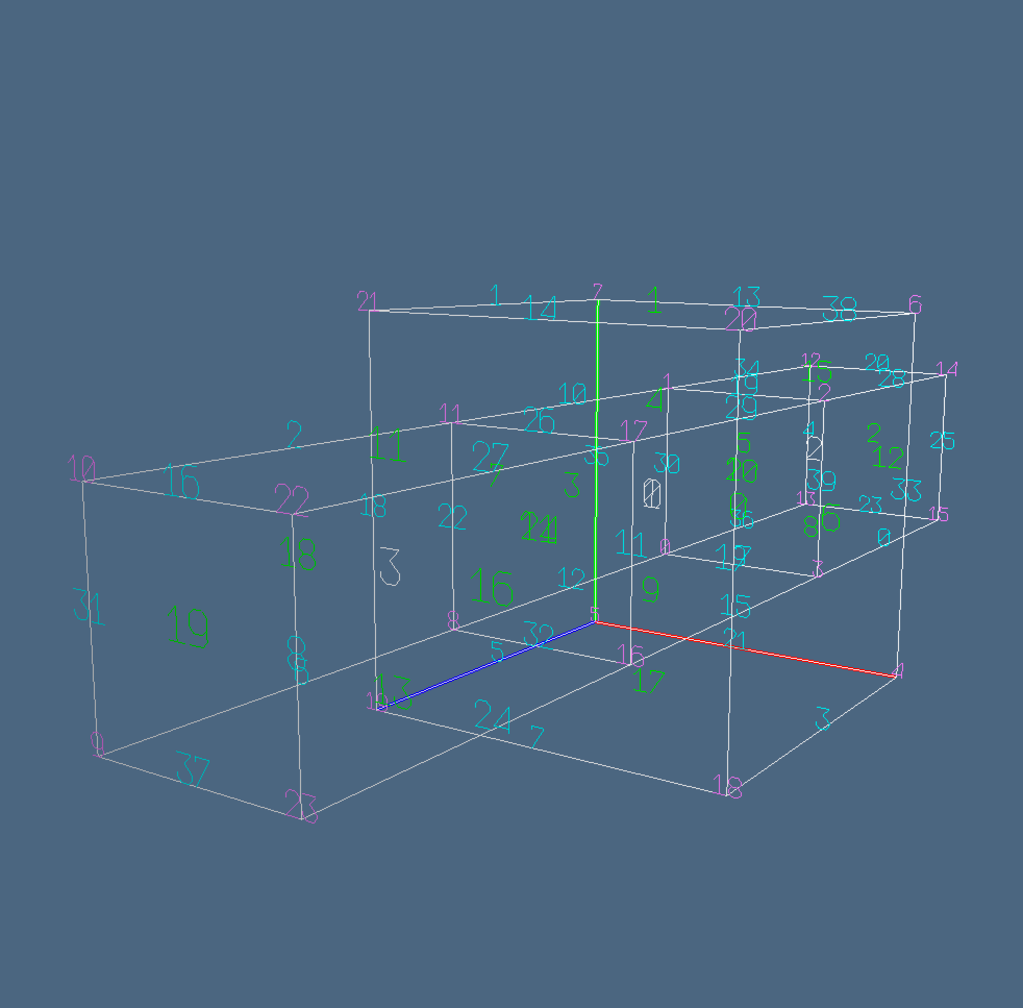
\includegraphics[height=0.495\linewidth,width=0.495\linewidth]{images/boundary-test03-1} 
   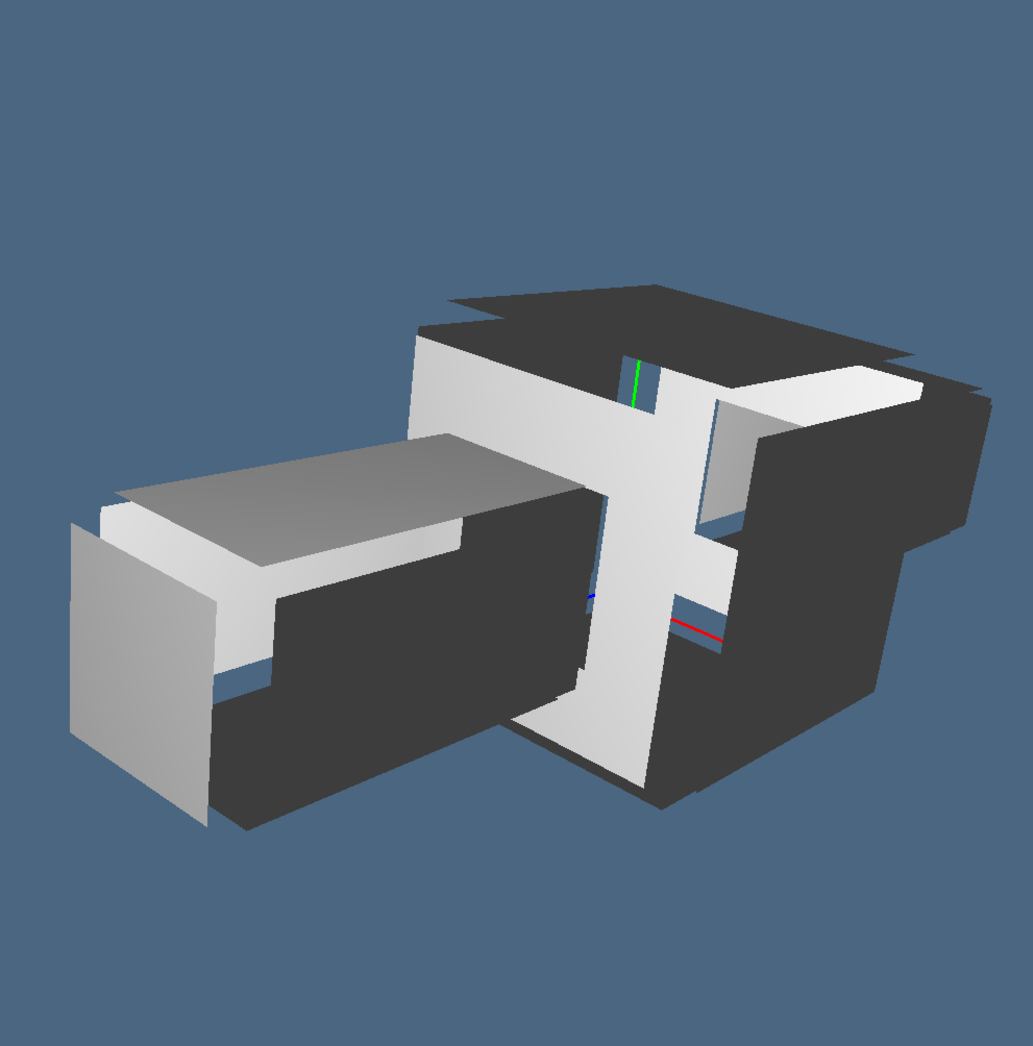
\includegraphics[height=0.495\linewidth,width=0.495\linewidth]{images/boundary-test03-2} 
   \caption{Non-convex 3-complex. (a) Indexing of 0-,1-,2- and 3-cells; (b) exploded 2-boundary cells.
   Notice that two faces are multiply-connected.}
   \label{fig:boundary-test03}
\end{figure}


\begin{figure}[htbp] %  figure placement: here, top, bottom, or page
   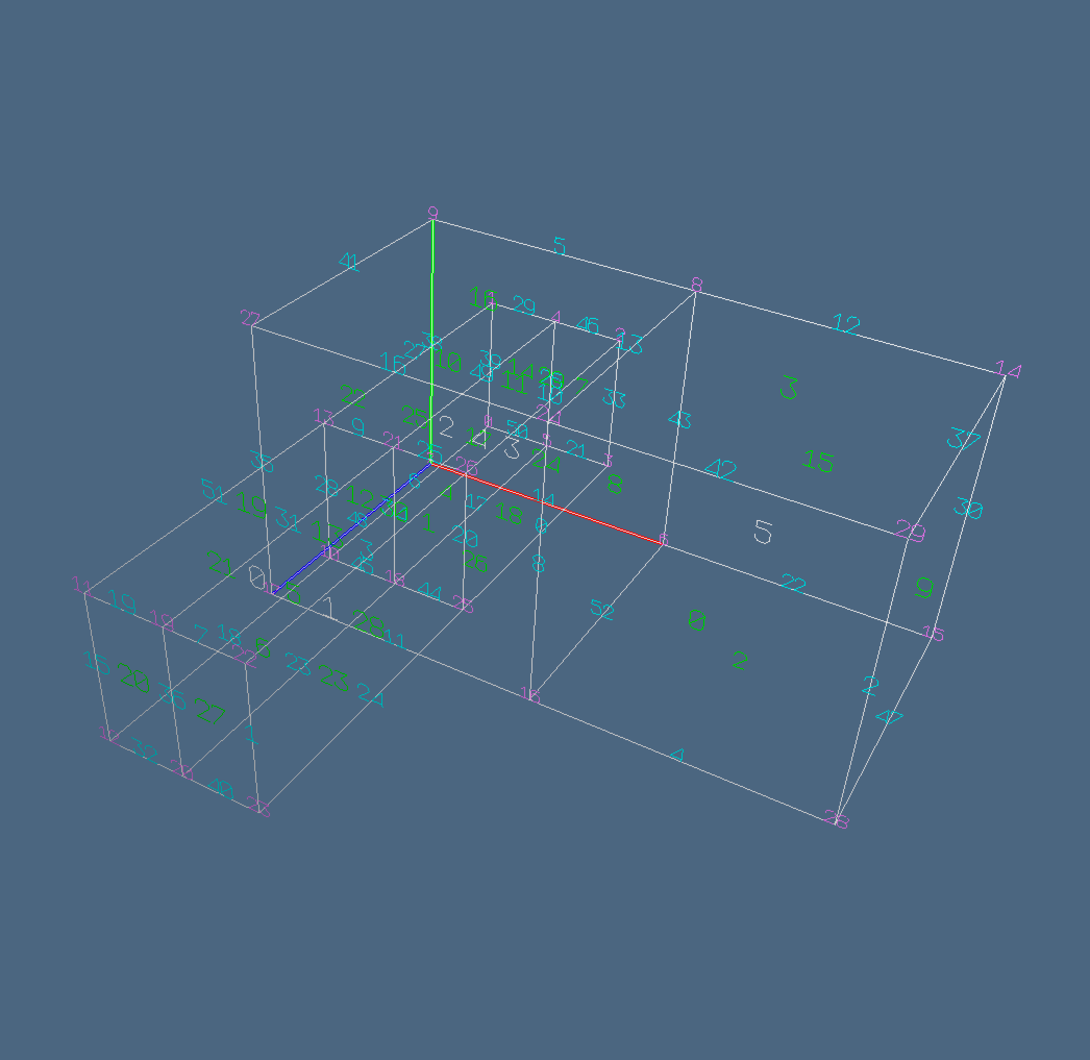
\includegraphics[height=0.245\linewidth,width=0.245\linewidth]{images/boundary-test04-1} 
   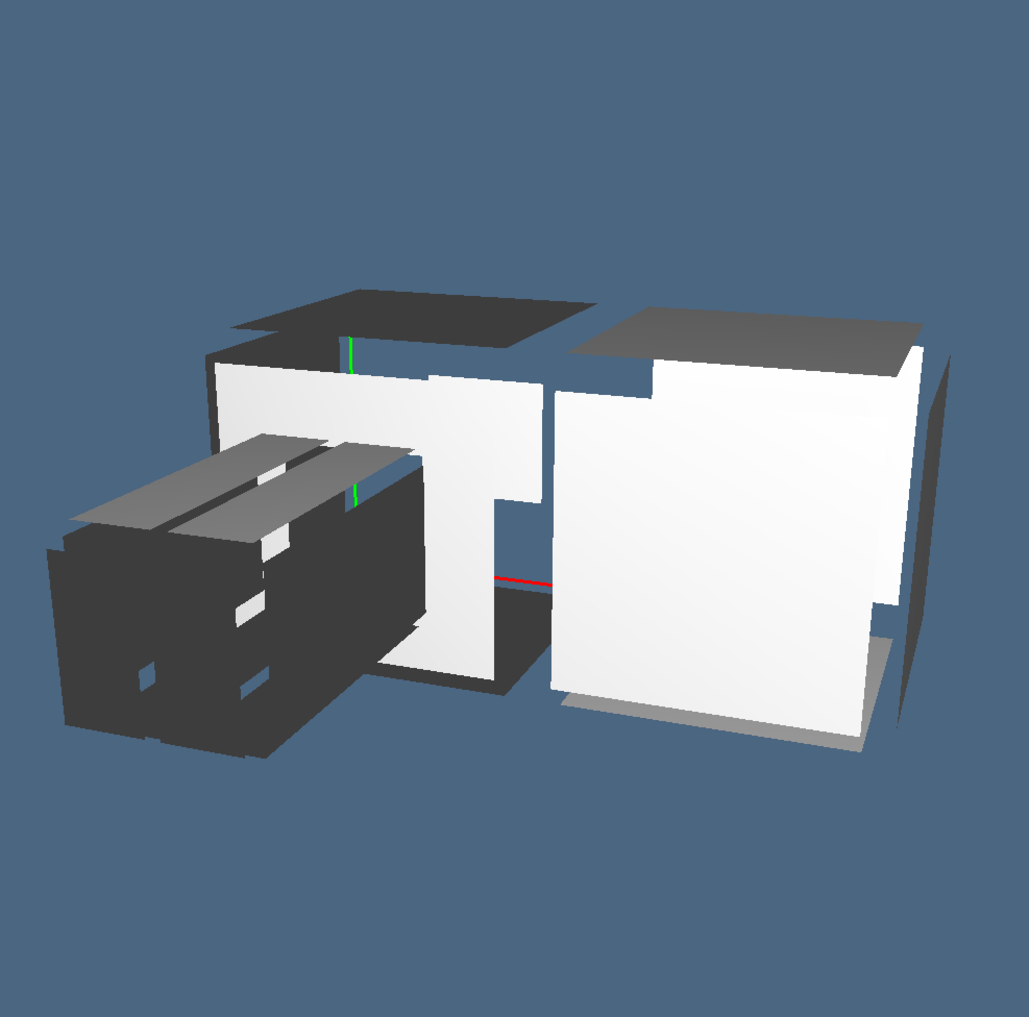
\includegraphics[height=0.245\linewidth,width=0.245\linewidth]{images/boundary-test04-2} 
   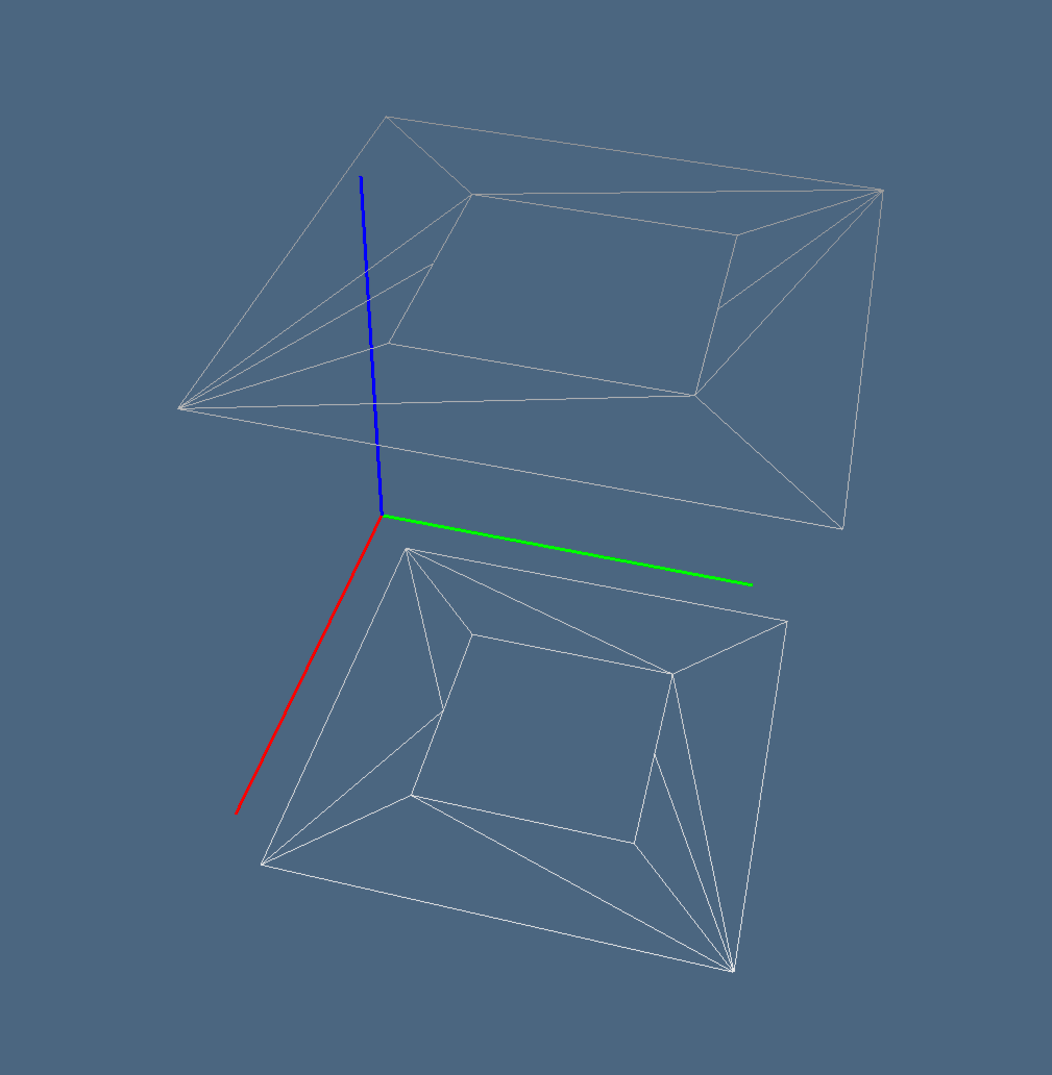
\includegraphics[height=0.245\linewidth,width=0.245\linewidth]{images/boundary-test03-4} 
   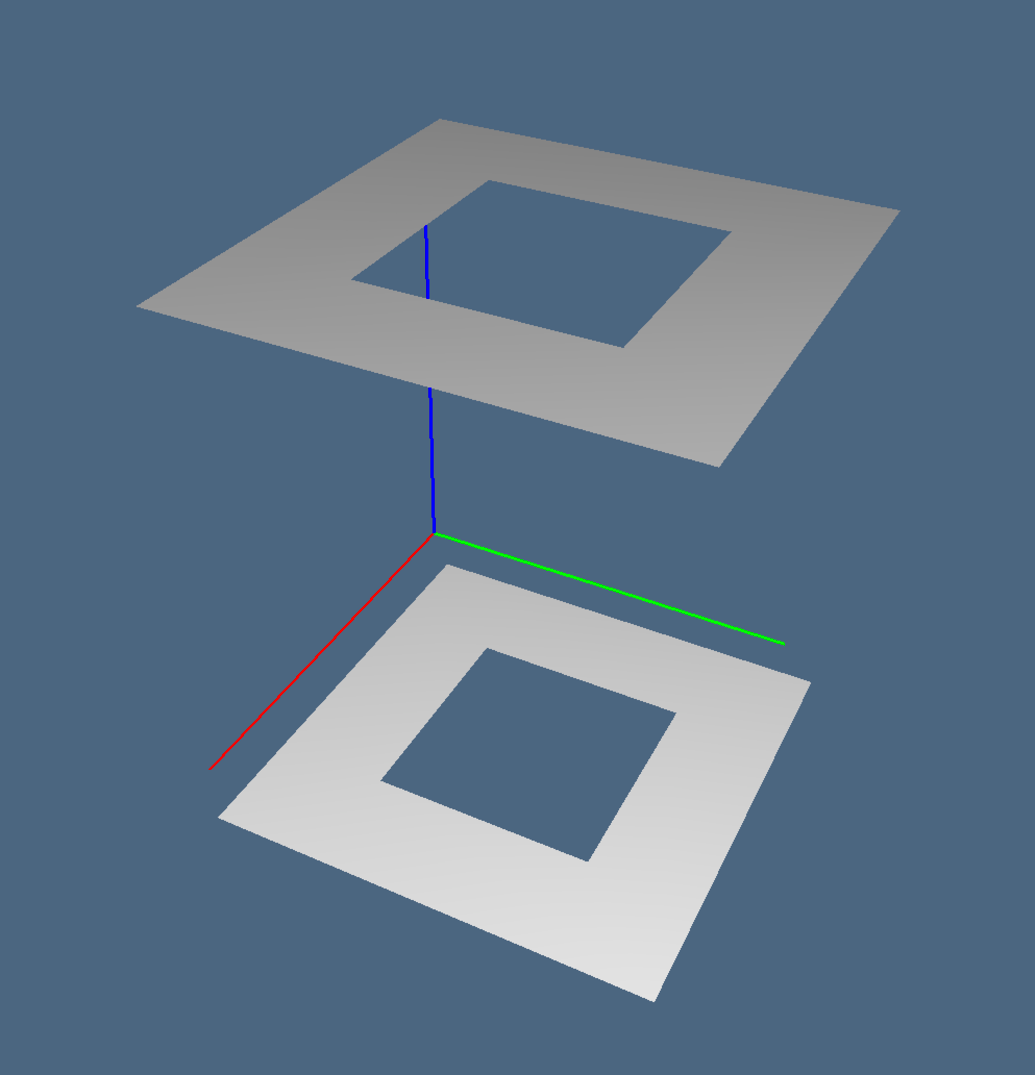
\includegraphics[height=0.245\linewidth,width=0.245\linewidth]{images/boundary-test03-5} 
   \caption{Non-convex 3-complex. (a) Indexing of 0-,1-,2- and 3-cells; (b) exploded 2-boundary cells ---notice a drawing error on the back of the model---conversely, the data structures involved are correct, as shown by the two following pictures;
   (c) solid drawing of the 2-chain \texttt{[FV[29],FV[30]]}; (d) triangulation of the same 2-chain.}
   \label{fig:boundary-test04}
\end{figure}

\paragraph{3D non-convex LAR cells}
In this example the 3D model is constructed partly in automated way, partly by hand.
In particular, first we generate a structure of cuboidal complexes, then we transform it is a single complex using part of the computational pipeline being developed for the Boolean arrangments of complexes, so that all the included cells are mutually fragmented. Then the 3-cells are assembed as sets of 2-faces, giving the \texttt{CF} (cells-by-faces) variable. Finally this one is transformed automatically into \texttt{CV} (cells-by-vertices).

%-------------------------------------------------------------------------------
@O test/py/boundary/test04.py
@{""" 3D non-convex LAR cells """
from larlib import *
@< Input of a cellular 3-complex @>
@< Visualization of a 2-chain of a 3-complex @>
@< Visualization of a 3-chain of a 3-complex @>
@}
%-------------------------------------------------------------------------------

\paragraph{Input of a cellular 3-complex}
%-------------------------------------------------------------------------------
@D Input of a cellular 3-complex
@{""" Input of a cellular 3-complex """
V,[VV,EV,FV,CV] = larCuboids([2,1,1],True)
struct = Struct([(V,FV,EV),t(.25,.25,0),s(.25,.5,2),(V,FV,EV)])

V,FV,EV = struct2Marshal(struct)
CF = AA(sorted)([[20,12,21,5,19,6],[27,1,5,28,13,23],[12,14,25,17,10,4],
[1,7,17,24,11,18],[30,29,26,16,8,22,10,11,4,18,24,25],[2,3,8,9,0,15]])
CV = [list(set(CAT([FV[f]  for f in faces]))) for faces in CF]

VV = AA(LIST)(range(len(V)))
hpc = STRUCT(MKPOLS((V,EV)))
VIEW(larModelNumbering(1,1,1)(V,[VV,EV,FV,CV],hpc,0.6))
@}
%-------------------------------------------------------------------------------


\paragraph{Visualization of a 2-chain of a 3-complex}
%-------------------------------------------------------------------------------
@D Visualization of a 2-chain of a 3-complex
@{""" Visualization of the boundary 2-chain of a 3-complex """

"""
V,BF,BE = larUnsignedBoundary3(V,CV,FV,EV)(len(CV)*[1])
VIEW(STRUCT(MKTRIANGLES((V,BF,EV),color=True)))
VIEW(SKEL_1(STRUCT(MKTRIANGLES((V,BF,EV)) )))

boundaryEdges = chain2BoundaryChain(larUnsignedBoundary2(FV,EV,VV))
edgeChain = boundaryEdges(29*[0]+[1]+[1]) 
VIEW(EXPLODE(1.2,1.2,1.2)(MKTRIANGLES((V,FV[29:31],[EV[e] for e in edgeChain]),color=True)))
VIEW(SKEL_1(EXPLODE(1.2,1.2,1.2)(MKTRIANGLES((V,FV[29:31],[EV[e] for e in edgeChain])))))
"""
@}
%-------------------------------------------------------------------------------

\paragraph{Visualization of a 3-chain of a 3-complex}
%-------------------------------------------------------------------------------
@D Visualization of a 3-chain of a 3-complex
@{""" Visualization of a 3-chain of a 3-complex """

print "\n****** ECCOMI"
V,BF,BE = larUnsignedBoundary3(V,CV,FV,EV)([0,0,0,0,1,1])
VIEW(STRUCT(MKTRIANGLES((V,BF,BE))))
VIEW(SKEL_1(STRUCT(MKTRIANGLES((V,BF,BE)) )))
@}
%-------------------------------------------------------------------------------


%-------------------------------------------------------------------------------
@O test/py/boundary/test05.py
@{""" Boundary of a 3-complex """
from larlib import *

V,[VV,EV,FV,CV] = larCuboids([1,1,1],True)
cube = Struct([ (V,FV,EV) ])
assembly = Struct([ cube, Struct([t(0,.5,0), r(PI/4,0,0), s(.5,.5,.5),cube]) ])

V,FV,EV = struct2Marshal(assembly)
VV = AA(LIST)(range(len(V)))
hpc = STRUCT(MKPOLS((V,EV)))
VIEW(larModelNumbering(1,1,1)(V,[VV,EV,FV],hpc,0.6))

CF = [[1,2,3,4,6,7],[0,1,2,3,4,5,6,7,8,9,10,11]]
CV = [list(set(CAT([FV[f]  for f in faces]))) for faces in CF]

V,BF,BE = larUnsignedBoundary3(V,CV,FV,EV)([0,1])
VIEW(EXPLODE(1.2,1.2,1.2)(MKTRIANGLES((V,BF,BE),color=True))) 
@}
%-------------------------------------------------------------------------------

%-------------------------------------------------------------------------------
@O test/py/boundary/test06.py
@{""" Boundary of a 3-complex """
from larlib import *

V,[VV,EV,FV,CV] = larCuboids([1,1,1],True)
cube = Struct([ (V,FV,EV) ])
hole = Struct([t(0,.5,0), r(PI/4,0,0), s(.5,.5,.5),cube])
assembly = Struct([ cube, hole, t(0,0,SQRT(0.5)), hole ])

V,FV,EV = struct2Marshal(assembly) # WRONG:  TODO: check ...
VV = AA(LIST)(range(len(V)))
hpc = STRUCT(MKPOLS((V,EV)))
VIEW(larModelNumbering(1,1,1)(V,[[],[],FV],hpc,0.6))

CF = [[4,5,7,16,17,19,20],[3,8,6,12,11,13],[0,1,10,20],[]]
CV = [list(set(CAT([FV[f]  for f in faces]))) for faces in CF]

V,BF,BE = larUnsignedBoundary3(V,CV,FV,EV)([0,1,1,0])
VIEW(EXPLODE(1.2,1.2,1.2)(MKTRIANGLES((V,BF,BE)))) # ERROR in MKTRIANGLES with non-manifold face
VIEW(EXPLODE(1.2,1.2,1.2)(MKFACES((V,BF,EV))))
VIEW(SKEL_1(EXPLODE(1.2,1.2,1.2)(MKFACES((V,BF,EV)))))
@}
%-------------------------------------------------------------------------------

%-------------------------------------------------------------------------------
@O test/py/boundary/test07.py
@{""" Boundary of a 3-complex """
from larlib import *

V,[VV,EV,FV,CV] = larCuboids([1,1,1],True)
cube = Struct([ (V,FV,EV) ])
hole = Struct([t(0,.5,0), r(PI/4,0,0), s(1,.5/SQRT(2),.5/SQRT(2)),cube])
assembly = Struct([ cube, hole ])

V,FV,EV = struct2Marshal(assembly) # WRONG:  TODO: check ...
VV = AA(LIST)(range(len(V)))
hpc = STRUCT(MKPOLS((V,EV)))
VIEW(larModelNumbering(1,1,1)(V,[VV,EV,FV],hpc,0.6))

CF = [[1,3,6,7,12,11],[0,2,4,5,9,8]]
CV = [list(set(CAT([FV[f]  for f in faces]))) for faces in CF]

V,BF,BE = larUnsignedBoundary3(V,CV,FV,EV)([1,0])
VIEW(EXPLODE(1.2,1.2,1.2)(MKTRIANGLES((V,BF,EV),color=True)))
@}
%-------------------------------------------------------------------------------


%-------------------------------------------------------------------------------
@O test/py/boundary/test08.py
@{""" Boundary of a 3-complex """
from larlib import *

V,[VV,EV,FV,CV] = larCuboids([1,1,1],True)
cube = Struct([ (V,FV,EV) ])
hole = Struct([t(0,.5,0), r(PI/4,0,0), s(1,.5/SQRT(2),.5/SQRT(2)),cube])
assembly = Struct([ cube, hole ])
assembly2 = Struct([ assembly, t(0,0,.5), s(0.5,1,1), hole ])

V,FV,EV = struct2Marshal(assembly2) 
VV = AA(LIST)(range(len(V)))
hpc = STRUCT(MKPOLS((V,EV)))
VIEW(larModelNumbering(1,1,1)(V,[VV,EV,FV],hpc,0.7))

#CF = [[1,3,6,14,17,18,19, 0,4,9,11,15,16, 2,5,7,8,10,13],[0,4,9,11,15,16],[2,5,7,8,10,13]]
CF = [[16,9,11,0,15,4],[10,12,7,2,17,15,9,5,18,8,16,3,6,14,19,4,1],[5,13,7,10,8,2]]
CV = [list(set(CAT([FV[f]  for f in faces]))) for faces in CF]

n = len(CV)
for k in range(n): 
    V,BF,BE = larUnsignedBoundary3(V,CV,FV,EV)(IDNT(n)[k])
    VIEW(STRUCT(MKTRIANGLES((V,BF,BE),color=True))) 
    VIEW(EXPLODE(1.2,1.2,1.2)(MKTRIANGLES((V,BF,BE),color=True))) 
    VIEW(SKEL_1(EXPLODE(1.2,1.2,1.2)(MKTRIANGLES((V,BF,BE)))))
V,BF,BE = larUnsignedBoundary3(V,CV,FV,EV)([1,1,1])
VIEW(SKEL_1(EXPLODE(1.2,1.2,1.2)(MKTRIANGLES((V,BF,BE)))))
@}
%-------------------------------------------------------------------------------

\begin{figure}[htbp] %  figure placement: here, top, bottom, or page
   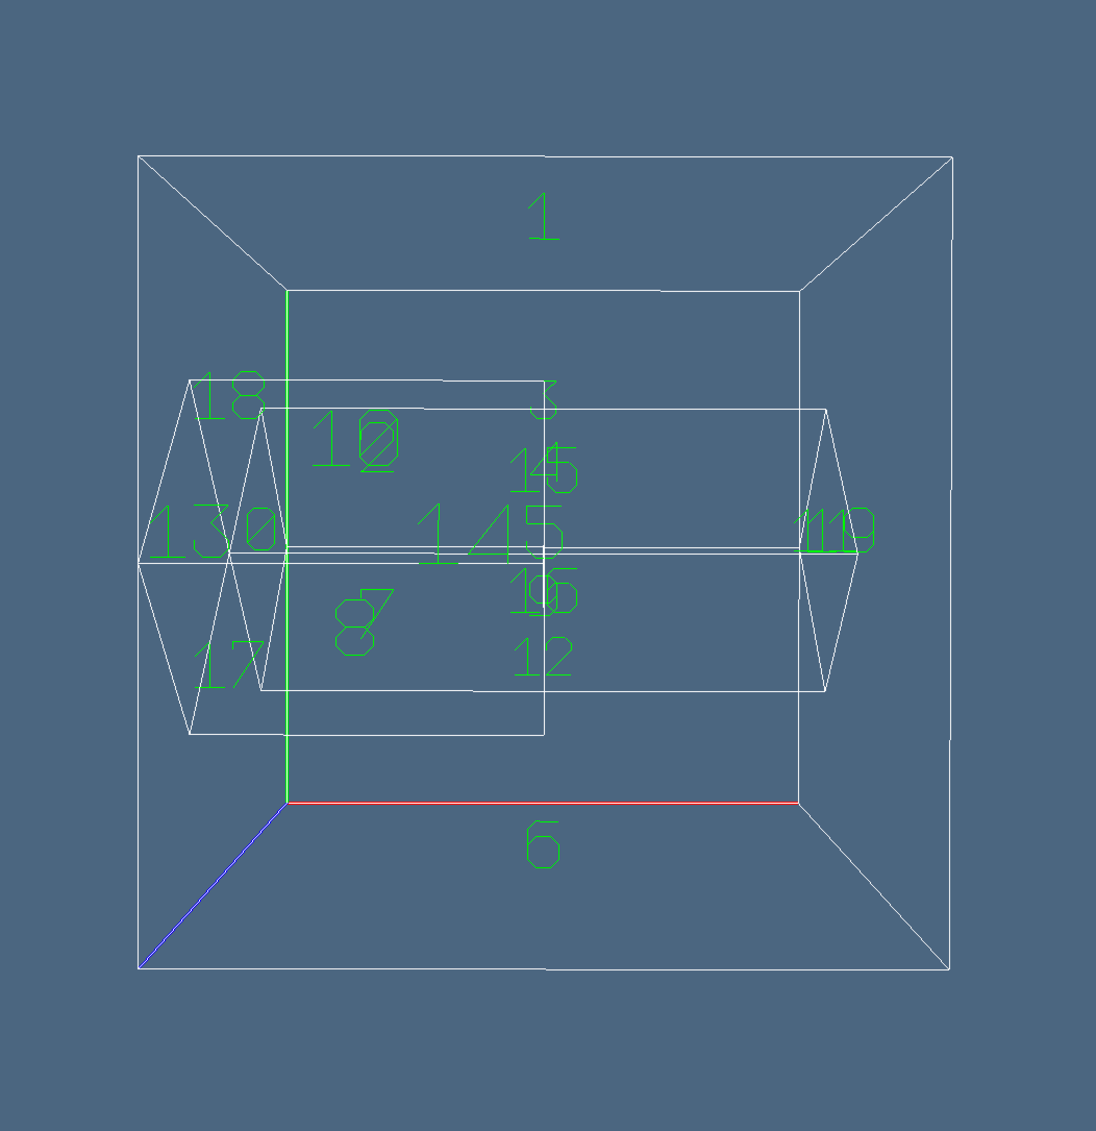
\includegraphics[height=0.245\linewidth,width=0.245\linewidth]{images/topos1} 
   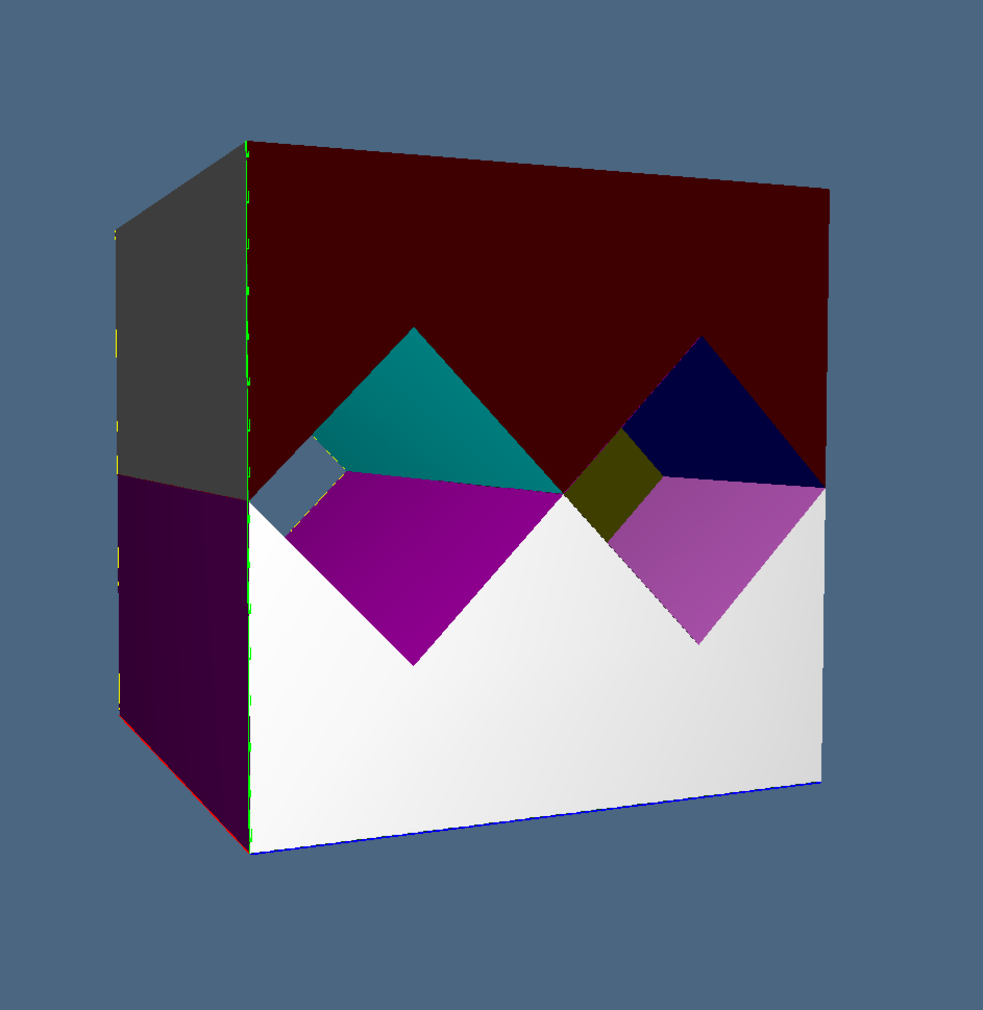
\includegraphics[height=0.245\linewidth,width=0.245\linewidth]{images/topos2} 
   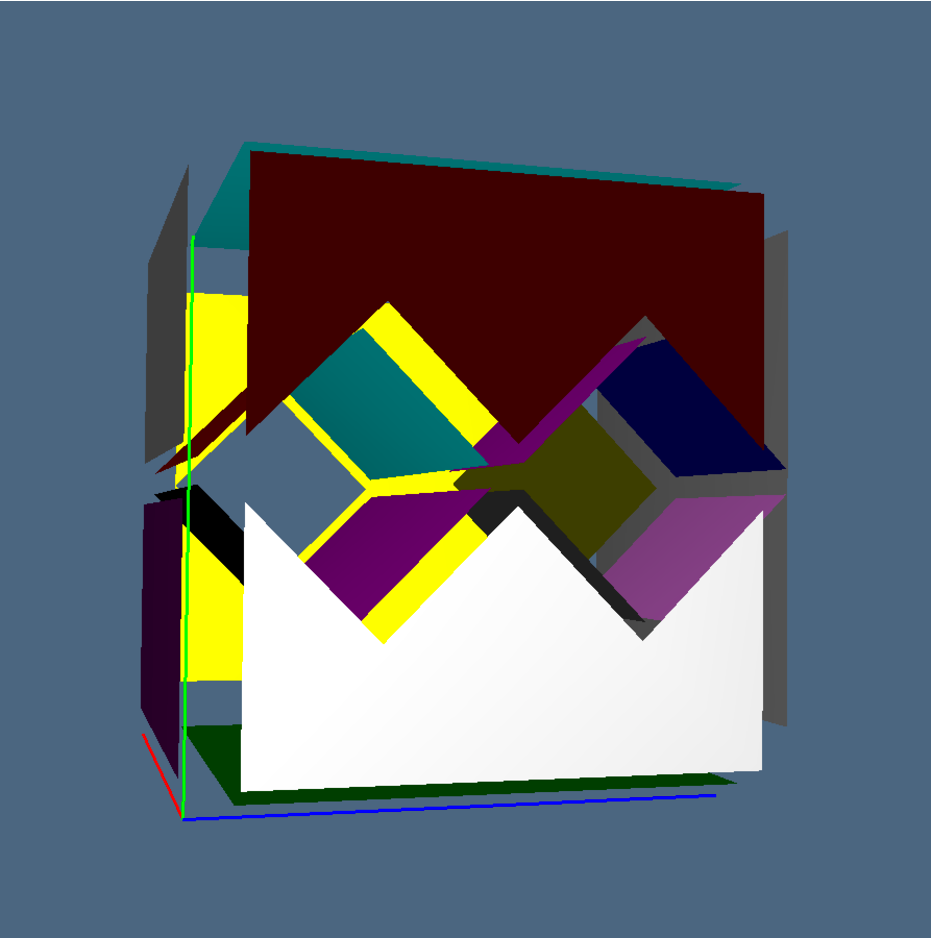
\includegraphics[height=0.245\linewidth,width=0.245\linewidth]{images/topos3} 
   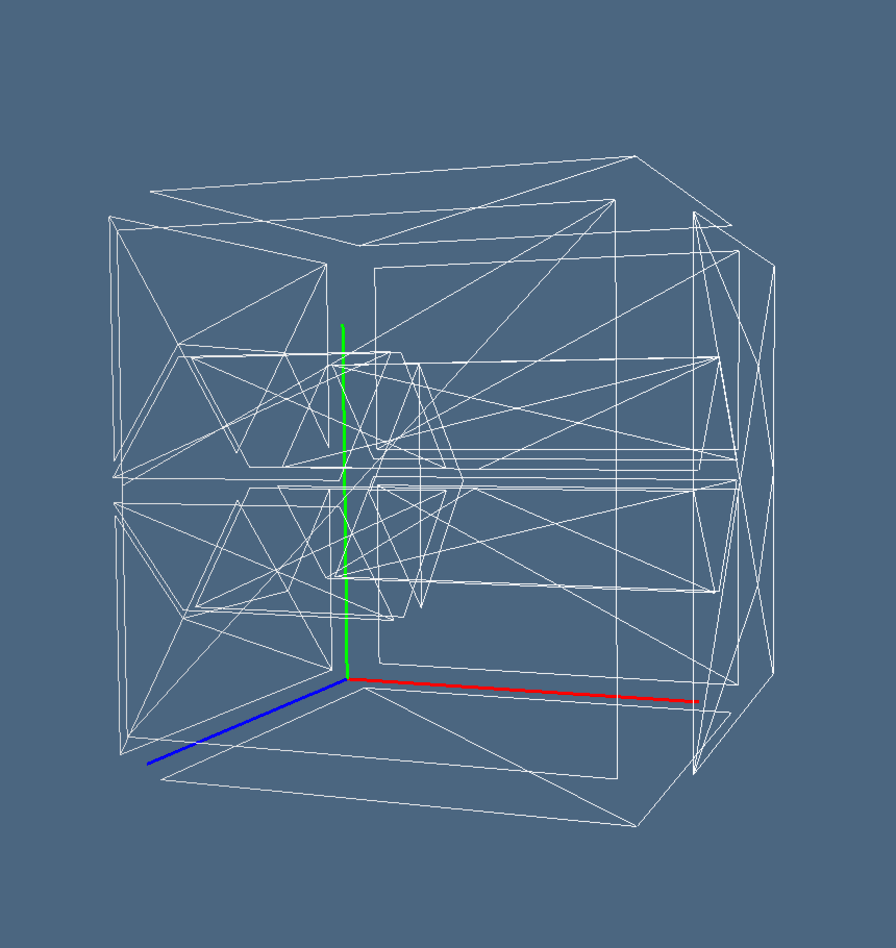
\includegraphics[height=0.245\linewidth,width=0.245\linewidth]{images/topos4} 
   \caption{Decomposition of the unit 3-cube in a cellular 3-complex with three 3-cells. Two 3-cells are homeomorphic to the 3-ball, while the remaining one is homeomorphic to the 3-torus.
Notice that one of 2-cells (as well one of 3-cells) are non-contractible and non-manifold, as well as non-convex:
   (a) Indexing of 2-faces of the 3-complex; (b) drawing of the (boundary of) non-convex 3-cell;
   (c) exploded drawing of the (boundary of) non-convex 3-cell; (d) triangulation of its 2-faces.
   The triangulation of LAR 2-faces is needed in order to draw them solidly.}
   \label{fig:boundary-test04}
\end{figure}




\appendix
\section{Utilities}


\paragraph{Marshalling a structure to a LAR cellular model}
The function \texttt{struct2Marshal} transforms a \texttt{Struct} object, often used to 
define some assembly of simpler models, to a correctly defined LAR cellular model, i.e.~to
a cellular partition of the space, in other words a quasi-disjoint partition of the object into well-glued cells of suitable dimensions.

%-------------------------------------------------------------------------------
@D Marshalling a structure to a LAR cellular model
@{""" Marshalling a structure to a LAR cellular model """
import boolean,inters

def struct2Marshal(struct):
    W,FW,EW = struct2lar(struct)
    quadArray = [[W[v] for v in face] for face in FW]
    parts = boolean.boxBuckets3d(boolean.containmentBoxes(quadArray))
    Z,FZ,EZ = boolean.spacePartition(W,FW,EW, parts)
    V,FV,EV = inters.larSimplify((Z,FZ,EZ),radius=0.001)
    return V,FV,EV
@}
%-------------------------------------------------------------------------------

\paragraph{Boundary of a 3-complex}
%-------------------------------------------------------------------------------
@D Boundary of a 3-complex
@{""" Boundary of a 3-complex """
import larcc
"""  WHY wrong ????  TOCHECK !!
def larUnsignedBoundary3(V,CV,FV,EV):
    VV = AA(LIST)(range(len(V)))
    operator3 = larcc.chain2BoundaryChain(boundary3(CV,FV,EV))
    operator2 = larcc.chain2BoundaryChain(larUnsignedBoundary2(FV,EV,VV))
    def larUnsignedBoundary30(chain):
        BF = operator3(chain)
        faceCoords = len(FV)*[0]
        for f in BF: faceCoords[f] = 1
        BE = operator2(faceCoords)
        return V,[FV[f] for f in BF],[EV[e] for e in BE]
    return larUnsignedBoundary30
"""
def larUnsignedBoundary3(V,CV,FV,EV):
    VV = AA(LIST)(range(len(V)))
    operator3 = larcc.chain2BoundaryChain(boundary3(CV,FV,EV))
    operator2 = larcc.chain2BoundaryChain(larUnsignedBoundary2(FV,EV,VV))
    def larUnsignedBoundary30(chain):
        BF = operator3(chain)
        BE = set()
        for f in BF: 
            faceCoords = len(FV)*[0]
            faceCoords[f] = 1
            BE = BE.union(operator2(faceCoords))
        return V,[FV[f] for f in BF],[EV[e] for e in BE]
    return larUnsignedBoundary30
@}
%-------------------------------------------------------------------------------


\begin{figure}[htbp] %  figure placement: here, top, bottom, or page
   \centering
   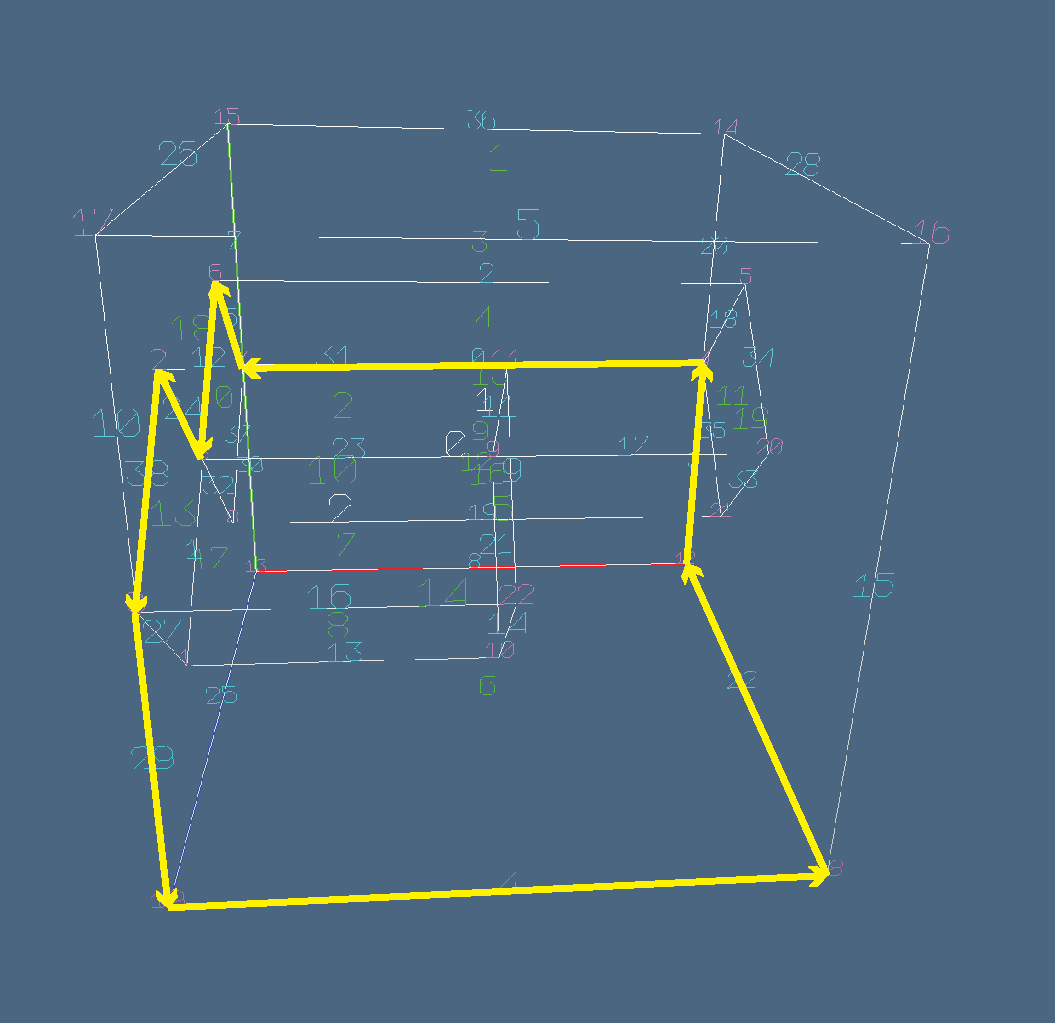
\includegraphics[width=0.5\linewidth]{images/edgecycle} 
   \caption{The oriented boundary 1-cycle of a partial 3-cell extraction from a 2-complex in 3D.}
   \label{fig:edgecycle}
\end{figure}


\bibliographystyle{amsalpha}
\bibliography{boundary}


\end{document}
